 \documentclass[12pt,letterpaper]{article}

%packages
% NC: Just to flag here how I'll comment on LaTeX files. I'll use % and then NC. Of course in git diff it'll all show up as an addition.
% NC: You could add all the packages etc to a template .sty file to save writing it all up here. Rich's ms.sty that I provided on DropBox is a good example

% TG: Just a general note for the file outline: I write every sentence of a same paragraph on a new line, no real reason for that appart that I can then see when the sentence is way to long. Also, I kept the big hidden headers ("%----") that you don't seem to like, without them it totally wrecks my head to know how much do I still have to scroll...

\usepackage{fixltx2e}
\usepackage{textcomp}
\usepackage{fullpage}
%\usepackage{nag}
\usepackage{natbib}
%\usepackage{bibtex}
\usepackage{float}
\usepackage{latexsym}
%\usepackage{hyperref} 
\usepackage{url}
%\usepackage{html}
\usepackage{hyperref}
\usepackage{epsfig}
\usepackage{graphicx}
\usepackage{amssymb}
\usepackage{amsmath}
\usepackage{bm}
\usepackage{array}
\usepackage[version=3]{mhchem}
\usepackage{ifthen}
\usepackage{caption}
\usepackage{hyperref}
%\usepackage{xcolor}
\usepackage{amsthm}
\usepackage{amstext} % Add and remove packages as necessary for your manuscript.

% NC: Added by NC
\usepackage{enumerate}
\usepackage[osf]{mathpazo} % palatino is a nicer font! 
\pagenumbering{arabic} % Page numbers

%Pagination style and stuff
\linespread{1.66} % All text should be double-spaced with occasional exceptions for tables. 
\raggedright
\setlength{\parindent}{0.5in}

\setcounter{secnumdepth}{0} % Our sections are not numbered and our papers do not have Tables of Contents. We don't present a list of figures or list of tables, either. Any common font is fine. (A common sans-serif font should be used on figures, but figures should be separate from the LaTeX document.)

%\pagestyle{empty}

\renewcommand{\section}[1]{%
\bigskip
\begin{center}
\begin{Large}
\normalfont\scshape #1
\medskip
\end{Large}
\end{center}}

\renewcommand{\subsection}[1]{%
\bigskip
\begin{center}
\begin{large}
\normalfont\itshape #1
\end{large}
\end{center}}

\renewcommand{\subsubsection}[1]{%
\vspace{2ex}
\noindent
\textit{#1.}---}

\renewcommand{\tableofcontents}{}

\bibpunct{(}{)}{;}{a}{}{,}  % this is a citation format command for natbib


%---------------------------------------------
%
%       START
%
%---------------------------------------------

\begin{document}

%For a colour version of the draft to a search>replace '-BW'>'' 
%\modulolinenumbers[1]     % Line numbering on every line

%Running head
\begin{flushright}
Version dated: \today
\end{flushright}
\bigskip
\noindent RH: Missing data and topology in total evidence approach %RH = Running Head

\bigskip
\medskip
\begin{center}

%Title
\noindent{\Large \bf Effect of missing data on correct topological recovery using a total evidence approach}
%Alternative punchier title: "Bayesian Total Evidence methods fail to recover correct topologies from matrices containing both living and fossil taxa"
%Alternative punchier title: "Maximum Likelihood outperforms Bayesian methods for inferring topology from Total Evidence matrices containing both living and fossil taxa"
% NC: Not sure about any of these. I actually think I prefer your talk title. So something like: The effects of missing data on the ability of Total Evidence approaches to recover correct tree topologies. No rush to decide. But needs Total Evidence in there somewhere.

\bigskip

%Authors
% TG: For the authorship, we can always squeeze whoever wants to be in the paper between the two of us. However, following the rule "Should I be author? Yes if I can give a talk about the paper." I think that just leaves the two of us.
\noindent {\normalsize \sc Thomas Guillerme$^1$$^,$$^2$, and Natalie Cooper$^1$$^,$$^2$}\\
\noindent {\small \it 
$^1$School of Natural Sciences, Trinity College Dublin, Dublin 2, Ireland;\\
$^2$Trinity Centre for Biodiversity Research, Trinity College Dublin, Dublin 2, Ireland;}\\
\end{center}
\medskip
\noindent{\bf Corresponding author:} Thomas Guillerme, School of Natural Sciences, Trinity College Dublin, Dublin 2, Ireland; E-mail: guillert@tcd.ie; Fax: +353 1 6778094; Tel: +353 1 896 2571.\\
\vspace{1in}

%---------------------------------------------
%
%       ABSTRACT
%
%---------------------------------------------

\newpage
\begin{abstract}
% NC: I'm not going to give this much work as it'll change before we submit anyway. Note though that and abstract must NOT just repeat stuff in the intro. Needs rephrasing at the very least.
Living species represent less than 1\% of all species that have ever lived. % NC: I was chatting to Andy Purvis about this the other day and he said lots of palaeo folk hate that stat. So let's not start the abstract with it!
Ignoring fossil taxa may lead to misinterpretation of macroevolutionary patterns and processes such as trends in species richness, biogeographical history or paleoecology.
This fact has led to an increasing consensus among scientists that both living and fossil taxa must be included in macroevolutionary studies.
One approach, the Total Evidence approach, uses molecular data from living taxa and morphological data from both living and fossil taxa to infer phylogenies with both living and fossil taxa at the tips.
Although the Total Evidence approach seems very promising, it requires a lot of data and is therefore likely to suffer from missing data issues which may affect its ability to infer correct phylogenies.

In this study we assess the effect of missing data on tree topologies inferred from Total Evidence matrices.
Using simulations we investigate three major factors that directly affect the completeness of the morphological part of the matrix:
(1) the proportion of living taxa with no morphological data,
(2) the amount of missing data in the fossil record, and
(3) the overall number of morphological characters in the matrix.
We find that, in a Bayesian framework, difficulties in recovering a stable topology are mainly driven by the missing data in the molecular part of the matrix (for which fossil taxa have no data).
In a Maximum Likelihood framework, however, topology is not directly affected by missing data \textit{per se}, but by the number of morphological characters shared among the taxa.
Therefore, the two main drivers of incorrect topologies are the overall number of morphological characters and the number of living species with no morphological data.

Our results suggest that, in order to use Total Evidence approaches, one should reduce the missing data in the morphological part of the matrix for living species and use a Maximum Likelihood framework to fix the topology prior to the overall Bayesian phylogenetic inference process.
%More results!
\end{abstract}

\noindent (Keywords: missing data, Total Evidence, Bayesian, Maximum Likelihood, topology)\\

\vspace{1.5in}

\newpage 

%---------------------------------------------
%
%       INTRODUCTION
%
%---------------------------------------------

\section{Introduction}

Although most species that have ever lived are now extinct % NC: This avoids giving the dodgy stat of 1%
    \citep{novacek1992ext,raup1993extinction}, the majority of macroevolutionary studies focus solely on living species \citep[e.g.][]{meredithimpacts2011,jetzthe2012}. %or is citing of your own papers in the too "douchebagy" for the second sentence?
% NC: Yeah be careful with self citing. Fine if it's a good fit, but it's totally not here!!! A better citation would be a big biodiversity study, e.g. the bird phylogeny paper.
Ignoring fossil taxa may lead to misinterpretation of macroevolutionary patterns and processes such as the timing of diversification events \citep[e.g.][]{pyrondivergence2011}, relationships among lineages \citep[e.g.][]{manosphylogeny2007} or niche occupancy \citep[e.g.][]{pearmanniche2008}.
This has led to increasing consensus among scientists that fossil taxa must be included in macroevolutionary studies \citep{jacksonwhat2006,quentaldiversity2010,dietlconservation2011,slaterunifying2013,fritzdiversity2013}.
However, to do this we need to be able to place living and fossil taxa into the same phylogenies; a task that remains difficult despite recent methodological developments (e.g. \citealp{pyrondivergence2011,ronquista2012,schragocombining2013}). %Not a nice sentence

Up to now, three main approaches have been used to place both living and fossil taxa % NC: BE consistent. Either living and fossil, or fossil and living. - TG: Let's make it living and fossil then.
    into phylogenies.
These approaches differ mainly in whether they treat fossil taxa as tips or as nodes in the phylogeny, and in which part of the available fossil data is used (i.e. the age of the fossil only or both its age and morphology). % NC: Not sure about bit in brackets - TG: it's the idea of fossil occurence (age) only when node and fossil occurence + topology when tip.
Classical cladistic methods use matrices containing morphological data from both living and fossil taxa and treat each taxon as a tip in the phylogeny.
Relationships among the taxa are then inferred using optimality criteria such as maximum parsimony \citep{simpson1945}.
This approach is commonly used by paleontologists but it ignores the additional molecular data available from living species and does not allow use of probabilistic methods for dealing with phylogenetic uncertainty (but see \citealp{spencerefficacy2013}).
Neontologists, on the other hand, more commonly use probabilistic approaches (e.g. Maximum Likelihood or Bayesian methods) based on matrices containing only molecular data from living species.
Because fossil taxa do not usually have available DNA, fossils are used as nodes rather than tips in these phylogenies and their occurrence date % NC: Need to check the exact phrase needed here. Is it range of occurrence? Occurrence dates? etc. - TG: in paleo jargon we have FAD (first apparition datum) and FOD (first occurrence datum). FAD is always hypothetical (we can't really exactly know when the taxa appeared) and FOD is always subjective (it depends when the fossil was found, maybe next year someone will find another one in older layers). So for the dating, because it's relaxed clock, people use FOD (and also probably because they don't care since it doesn't make a huge difference I guess).
    are used to time calibrate phylogenies \citep{zuckerkandl1965}.
There have been great improvements in the theory and application of these two approaches \citep[e.g.][]{bapsta2013,stadlerdating2013,heaththe2013} as well as much debate about the "best" approach to use \citep[e.g.][]{spencerefficacy2013}.
However neither approach uses all the available data.

A final approach, known as the Total Evidence method, uses matrices containing molecular data from living taxa and morphological data from both living and fossil taxa \citep{eernissetaxonomic1993}. %There might be a philosophico-semantic distinction to do here. Is TEM a method or an approach? I'll say that it is an approach because it's more like an idea (put every thing together) than a way to do (how to put everything together). It makes more sense to me compared to a real method e.g. a probabilistic method such as ML where the method states precisely how to do stuff.
% NC: Tricky. Don't think it's too important though. 
% NC: I do think Total Evidence needs capital letters though, like ML and Bayesian - TG: fixed
This approach treats every taxon as a tip in the phylogeny, uses the occurrence age of the fossils to time calibrate the phylogeny, and allows the use of probabilistic methods for estimating phylogenetic uncertainty \citep{ronquista2012}.
Total Evidence methods have been successfully applied to empirical data \citep{pyrondivergence2011,ronquista2012,schragocombining2013}, and are becoming an increasingly popular way of adding fossil taxa to phylogenies.
However, although the Total Evidence approach seems very promising, there is one big drawback in using this approach: it requires a lot of data that can be difficult (or impossible) to collect.
%In particular it requires morphological data from both living and fossil taxa, both of which are known to be scarce. % NC: Really? I know fossil data is known to be scarce, but living data? I think people would be surprised. And they are surprised. We were surprised! Needs a citation either way.
%TG: how about this:
The morphological data for living taxa is rarely collected when molecular data is available (e.g. \citealt{O'Leary08022013} vs. \citealt{meredithimpacts2011}),% TG: i.e. in O'Leary they use meredith molecular data but only code few species from it.
 and, for fossil taxa, the scarcity of the fossil record only allow to collect the data available (for example, in vertebrates, the hardest parts of the skeleton; \citealt{sansomfossilization2013}).
Therefore Total Evidence matrices are likely to contain a lot of missing data that may affect the method's ability to infer correct topologies, branch lengths and support values \citep{salamin2003}. % Trevor: Missing data also influences support values that trend to decrease

% NC: You need to take a bit of time to learn about singular and plural grammar in English. It's something you always do wrong. e.g. The Total Evidence method *uses* this and *its* parameters are as follows. Versus: Total Evidence methods *use* this and *their* parameters are as follows. Sive and I won't be around to correct your English forever. - TG: my French demons are back!

The effect of missing data on phylogenetic inferences has been widely studied \citep{wiensmissing2003,wiensmissing2006,wiensmissing2008,lemmonthe2009,rouresite-specific2011,sansomfossilization2013,pattinsonphylogeny2014}.
Missing molecular data has been seen by some authors as an issue because it can, in some part of the tree, decrease phylogenetic signal (i.e. the evolutionary information contained within the matrix allowing to infer topology and branch length)% NC: define phylogenetic signal here. 
    , especially when using large matrices \citep{lemmonthe2009}.
However, this may not be a major issue because phylogenetic signal is easily increased by:
(i) including a "modest" number of highly-covered genes (i.e. approximatively of the genes that are coded for most of the species; \citealt{rouresite-specific2011}) %NC: what do you mean by highly-covered?
(ii) adding a greater number of taxa (especially slowly-evolving taxa or taxa close to the outgroup; \citealt{rouresite-specific2011}); and
(iii) choosing more appropriate models of sequence evolution \citep{wiensmissing2006,wiensmissing2008,rouresite-specific2011}.
Similarly, missing morphological data might be seen as either a major or minor issue for accurately inferring phylogenies depending on the study in question \citep{wiensmissing2003,sansomfossilization2013,pattinsonphylogeny2014}.
Because soft-tissue characters are rarely preserved in the fossil record, missing data is mainly found in these characters, and is therefore not randomly distributed which can lead to biased placement of fossil taxa in phylogenies (e.g. \citeauthor{sansomfossilization2013} \citeyear{sansomfossilization2013} but see \citeauthor{pattinsonphylogeny2014} \citeyear{pattinsonphylogeny2014}).
However, the phylogenetic signal is not related to the amount of missing data \textit{per se} but to the number of informative characters for each taxon, therefore missing data is less of an issue than the number of shared informative characters \citep{wiensmissing2003}.
% NC: I'm a little dubious of what this paragraph is trying to get at in places. We should discuss at some point. TG: my idea was to do the "literature-review" part of the intro: missing data is already widely studied (answer to the comment: "hun... We already knew that") but it has never been studied in TEM framework. And that's kind of the point we're getting toward with our work: we don't really care about the effect of missing data per se (i.e. what's the threshold were it starts fucking up the phylogeny) but more the fact that Bayesian fails.

Although missing data does not appear be a major problem in molecular and morphological matrices separately \citep{wiensmissing2003,wiensmissing2006,wiensmissing2008,rouresite-specific2011}, it may become more of an issue in Total Evidence matrices containing both molecular and morphological data for living and fossil species.
This may be particularly problematic as fossil taxa (generally) do not have molecular data, resulting in a large section of missing data.
Until now, no attempt has been made to study the impact of this issue on phylogenetic inference from Total Evidence methods. 

% NC: Somewhere here you need to flag that you're only looking at topologies and briefly explain why.
In this study, we focused only on topology as one of the two aspects of the phylogenetic signal (topology and branch length).
Even though both aspects are equally important, branch topology is the first and most straightforward aspect reflecting phylogenetic signal (i.e. topological changes are discrete opposed to branch length changes are continuous).
Also, interestingly, the effect of Total Evidence method has not been formally assessed in previous studies using fixed topology \citep{ronquista2012,schragocombining2013}. %TG: or is that mean for them?

Here we use simulations to assess the effect of missing data on tree topologies inferred from Total Evidence matrices.
The molecular part of a Total Evidence matrix acts like a "classical" molecular matrix containing only the living taxa \citep{ronquista2012}.
The effect of missing data on such matrices is well known \citep{wiensmissing2006,wiensmissing2008,rouresite-specific2011}, therefore, we focus only on missing data in the morphological part of the matrix.
We investigate three major parameters that directly affect the completeness of the morphological part of the matrix:
\begin{enumerate}
\item the proportion of living taxa with no morphological data;
\item the proportion of missing data in the fossil taxa; and
\item the proportion of missing morphological characters for both living and fossil taxa in the matrix.
\end{enumerate}
We remove data from a Total Evidence matrix by changing the values of these three parameters and then assess how this affects the topology of trees inferred using Maximum Likelihood and Bayesian methods.
We chose these parameters because they reflect empirical biases in data availability.
The advent of molecular phylogenetics means that morphological data for living species is rarely collected, and few people have the skills to identify characters needed for detailed phylogenetic analysis.
Missing data in fossil taxa is very common due to preservation biases \citep{sansomfossilization2013}, and the overall number of characters depends on the effort of the people identifying them.
% NC: OK I'm not sure what the "real-life" reason for three is. - TG: fixed to "empirical" (or "practical" ?).
% TG: This paragraph is crap
% NC: I think it's fine!

We find that when using a Maximum Likelihood approach, as missing data increases, the likelihood of recovering the correct tree topology decreases.
However, even with no missing data, Total Evidence matrices dramatically reduce the performance of Bayesian methods for inferring tree topology.
We propose that this drastic difference between Bayesian and Maximum Likelihood methods is due to a flattening of the likelihood landscape caused by the unavoidable amount of missing molecular data for fossil taxa in a Total Evidence matrix.
We make suggestions for how best to deal with this issue when inferring phylogenies from Total Evidence matrices.
% NC: You don't want to tell the whole story here. Just a results summary and a quick line of interpretation

%This problem leads to an inability of Bayesian chains to pick up the sub and near optimal topologies leading to high variance in the posterior tree distribution and really low support in the consensus tree.
%These results should encourage authors in not using Bayesian inference to explore the topological landscape of their phylogeny.
%Instead, we suggest that authors should first find the Maximum Likelihood tree and use it's topology as a fix prior in their Bayesian inference.
%We also propose a new method for comparing Bayesian posterior tree distribution's topology available in a wonderful R package. %Or am I just dreaming a bit too much here? 
% NC: Dreaming a bit much I think. There's a discussion to be had here about whether it's really a *new* method and whether you really want to make an R package per se. We definitely want to share the code

%-----------
% NC: It might look like I've done a lot to this but actually I think it's nearly there. A good thing to take from this is that writing a paper is *hard*. It gets easier, but it's still a deeply involved process with lots of writing and re-writing. Introductions are particularly difficult because if you don't set the scene, it's hard to convince people to get on board for the rest of the paper. This is why I said there was no way this was being submitted by the end of June! Still a long way to go I'm afraid in terms of time and effort. But that doesn't mean you're not doing well, *every* project is like this. 2 years is about average from conception to sending out a manuscript, and you only started work on this last spring.
%------------

%---------------------------------------------
%
%       METHODS
%
%---------------------------------------------


 
\newpage

\section{Methods} %no material needed?
% NC: Depends on the journal. See what Syst Biol asks for as section titles. TG: Syst Biol instructions :Elements vary, of course, depending on the type of paper. The first-level heading is often used for sections such as ``methods and materials,'' ``results,'' and' ``discussion;'' but other major sections are often appropriate instead.
To explore how missing data in the morphological sections of Total Evidence matrices influences tree topology, we used the following protocol (note that we explain each step in detail below this general outline; Fig.~\ref{Fig_Outline}). %NC: does Syst Biol use Fig. or Figure? - TG: it's "Fig." when it's a reference in brackets and "Figure" when it's a reference in the text. Table is always refered as "Table" (not "Tab").
\begin{enumerate}
\item{Generating the matrix} \label{step:generate_matrix} \\
We randomly generated a birth-death tree (hereafter called the "true" tree; Table ~\ref{Tab_glossary}) and used it to infer a matrix containing both molecular and morphological data for living and fossil taxa (hereafter called the "complete" matrix; Table ~\ref{Tab_glossary}).
\item{Removing data} \label{step:remove_data} \\
We removed data from the morphological part of the "complete" matrix to simulate the effects of missing data by modifying three parameters (i) the proportion of living taxa with no morphological data ($M_{L}$), (ii) the proportion of missing data in the fossil taxa ($M_{F}$) and (iii) the proportion of missing morphological characters ($M_{C}$) % NC: make sure to use the same descriptions here and in the introduction 
(the resulting matrices are called hereafter "missing-data" matrices; Table ~\ref{Tab_glossary}).
\item{Building phylogenies} \label{step:build_phylo} \\
We built phylogenetic trees from the "complete" matrix and from the "missing-data" matrices resulting in one tree generated from a matrix containing no missing data (hereafter called the "best" tree; Table ~\ref{Tab_glossary}) and multiple trees inferred from matrices with missing morphological data (hereafter called the "missing-data" trees; Table ~\ref{Tab_glossary}). Phylogenies were inferred via both Maximum Likelihood and Bayesian approaches.
\item{Comparing topologies} \label{step:compare_topo} \\
We compared the "best" tree to the "missing-data" trees to assess the influence of each parameter ($M_{L}$, $M_{F}$, $M_{C}$) and their interactions on the topologies of our phylogenies
\end{enumerate}
We repeated steps 1 to 4 50 times. %that's because I had 3 cluster accounts available... If it's a too odd number, no worries, I'll just remove the last chain.
% NC: Yeah 51 is odd. Let's just use 50.
A list of all the terms used in this paper is available in Table ~\ref{Tab_glossary}.

% NC: Not sure we need the glossary, but keep it for the thesis

\begin{table}[ht]
  \caption{Glossary}
  \centering
  \linespread{1.0}
  \begin{tabular}{p{5cm} p{9cm}}
\hline
\hfill Term & Definition \\[0.5ex]
\hline
\hfill living taxa & taxa with both molecular and morphological data available \\[1.5ex]
\hfill fossil taxa & taxa with only morphological data available \\[1.5ex]
\hfill "complete" matrix & matrix with no missing data except for the molecular part of the fossil taxa \\[1.5ex]
\hfill "missing-data" matrix & matrix with various amount of missing data \\[1.5ex]
\hfill $M_{L}$ & missing living taxa in the morphological part of the matrix \\[1.5ex]
\hfill $M_{F}$ & missing data for the fossil taxa in morphological part of the matrix \\[1.5ex]
\hfill $M_{C}$ & missing morphological characters for both living and fossil taxa \\[1.5ex]
\hfill "true" tree & tree used to simulate the matrix \\[1.5ex]
\hfill "best" tree & tree inferred from the "complete" matrix \\[1.5ex]
\hfill "missing-data" tree & tree inferred the "missing-data" matrices \\[1.5ex]
\hfill RPBTC & Random pairwise Bayesian tree comparison \\[1.5ex]
\hfill "horizontal" sub-matrix & sub-matrix with morphological and molecular characters for living taxa \\[1.5ex]
\hfill "vertical" sub-matrix & sub-matrix with morphological data for both living and fossil taxa \\[1.5ex]
\hfill "corner" sub-matrix & sub-matrix with morphological data for living taxa \\[1.5ex]
\hfill "missing-data" sub-matrix & molecular part of the matrix for the fossil taxa (no data) \\
\end{tabular} %Remove sub-matrices
  \label{Tab_glossary}
\end{table}


\begin{figure}
\centering
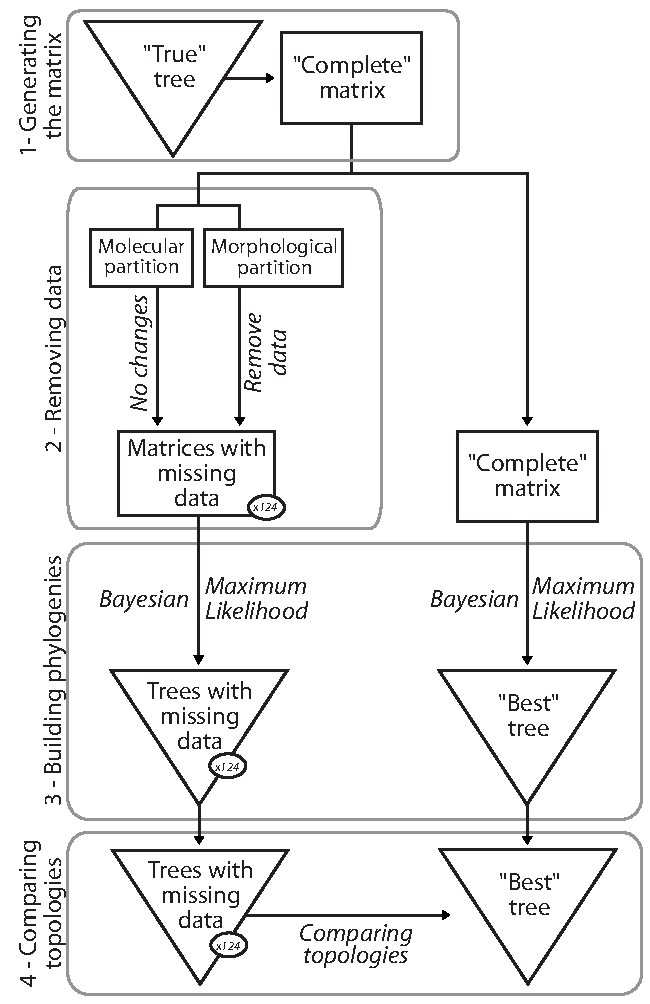
\includegraphics[keepaspectratio=true]{Figures/TEM_Fig_outline-BW.pdf}
\caption{Protocol outline.
(1) We randomly generated a birth-death tree (the "true" tree) and used it to infer a matrix with no missing data (the "complete" matrix).
(2) We removed data from the morphological part of the "complete" matrix resulting in 124 "missing-data" matrices.
% NC: I thought we had 124 missing data matrices... I just worked this out - one of the "missing data" matrices is 0%,0%,0% so = complete matrix. - TG: Yep, there is 125 matrices/trees per chain. 1 that's L00F00C00 and 124 others. It's again one of these habits like "adding missing data" that I have from the coding (that actually do add missing data and do generate 125 matrices).
(3) We built phylogenetic trees from each matrix using both Maximum Likelihood and Bayesian methods.
(4) We compared the "missing-data" trees to the "best" tree.
We repeated steps 1-4 50 times.}
\label{Fig_Outline}
\end{figure}

% NC: One tiny edit to the figure. I think the ML then Bayesian story is nice, so maybe change that part of the figure so it's ML then Bayesian. Also let's show this figure to a couple of people to see if they get it. -TG: Do you mean just swap the text ML/Bayesian (was: Bayesian-ML, is now: ML-Bayesian)?

%---------------------------------------------
%       Generating the matrix
%---------------------------------------------

% NC: Most of the below was fine but I've tried to condense it a bit as it's currently long even for Syst Biol. The key is to explain everything, but with minimal repetition.

\subsection{Generating the matrix}
First we randomly generated a "true" tree of 50 taxa in R v3.0.2 \citep{R302} using the package diversitree v0.9-6 \citep{fitzjohndiversitree2012}.
We generated the tree using a birth death process by sampling speciation ($\lambda$) and extinction ($\mu$) rates from a uniform distribution but maintaining $\lambda$ $>$ $\mu$ \citep{paradistime-dependent2011}.
We implemented a rejection sampling algorithm to select only trees with 25 living and 25 fossil taxa to ensure that we had enough taxa of each type for our missing data simulations to work.
We then added an outgroup to the tree, using the mean branch length of the tree to separate the outgroup from the rest of the taxa, and with the branch length leading to the outgroup set as the sum of the mean branch length and the longest root-to-tip length of the tree.

Next, we generated a molecular and a morphological matrix from the "true" tree.
The molecular matrix was inferred from the "true" tree using the R package phyclust v0.1-14 \citep{chen2011}.
The matrix contained 1000 character sites for 51 taxa and was generated using the seqgen algorithm \citep{ranbaut1997seqgen} and using the HKY model \citep{HKY85} with random base frequencies and transition/transversion rate of 2 \citep{douadycomparison2003}.
The substitution rates were distributed following a gamma distribution with an alpha ($\alpha$) shape of 0.5 \citep{yangamong-site1996}.
We chose a low value of $\alpha$ to reduce the number of sites with high substitution rates, thus avoiding too much homoplasy and a decrease in phylogenetic signal.
We selected the parameters above to generate data with no special assumption about how the characters evolved, and to reduce the computational time required if these parameters were estimated rather than defined in the tree building part of the analysis (even with the parameters defined, total computational time for the whole analysis was over 80 CPU years).
All the molecular information for fossil taxa was replaced by missing data ("?").

We inferred the morphological matrix using the R package ape v3.0-11 \citep{paradisape:2004} to generate a matrix of 100 character sites for 51 taxa.
We assigned the number of character states (either two or three) for each morphological character by sampling with a probability of 0.85 for two states characters and 0.15 for three state characters.
These probabilities were selected using the overall distribution of character states extracted from 100 published empirical morphological matrices (See \hyperref[supplementaries]{supplementaries}).
We then ran an independent discrete character simulation for each character using the "true" tree with the character's randomly selected number of states (two or three) and assuming an equal rate of change (i.e. evolutionary rate) from one character state to an other \citep{Pagel22011994}.
This method allows us to have only two parameters for each character: the number of states and the evolutionary rate.
For each character, the evolutionary rate was sampled from a gamma distribution with $\alpha$ = 0.5.
We used low evolutionary rate parameters (i.e. $\alpha$) to avoid homoplasy in the morphological part of the matrix and create a clear phylogenetic signal \citep{wagner2000,davalosintegrating2014}.

Finally, we combined the morphological and molecular matrices obtained from the "true" tree.
Hereafter we call this the "complete" matrix: the matrix with no missing data except for the molecular data of the fossil taxa.

%---------------------------------------------
%       Removing data
%---------------------------------------------

\subsection{Removing data}
We modified the "complete" matrix to get matrices with missing data by randomly replacing data with "?" in the morphological part of the matrices according to the following parameters (Fig. ~\ref{Fig_RemoveData}):

\begin{enumerate}
% NC: I'm not going to check but make sure the brief explanations of the parameters here are the same as in the intro and outline above. Also look at my justifications in the intro too. I think this may need a bit more justification as it's the main part of your simulations.
\item{The proportion of living taxa with no morphological data ($M_{L}$): 0\%, 10\%, 25\%, 50\% or 75\%.}
This parameter illustrates the number of living taxa that are present in the molecular part of the matrix but not in the morphological part.
This reflects the fact that because of the increasing availability of DNA sequences for living taxa, detailed morphological data is scarce.
\item{The proportion of missing data in the fossil taxa ($M_{F}$): 0\%, 10\%, 25\%, 50\% or 75\%.}
This parameter illustrates the quality of the fossil record. 
\item{the proportion of missing morphological characters for both living and fossil taxa ($M_{C}$): 0\%, 10\%, 25\%, 50\% or 75\%. }
This parameter illustrates the number of available morphological characters for both living and fossil taxa.
\end{enumerate}

% NC: I'm not sure this figure is helpful really. Let's test it on some people.
\begin{figure}
\centering
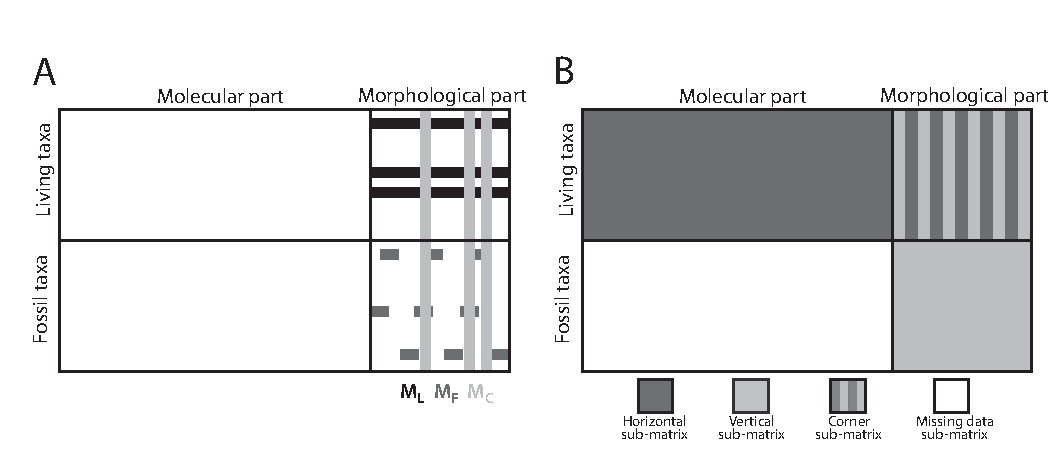
\includegraphics[keepaspectratio=true]{Figures/TEM_Fig_missingData-BW.pdf}
\caption{Names of the different parts of the matrix.
A: Missing data parameters:
Missing living - The proportion of living taxa with no morphological data ($M_{L}$);
Missing fossil - The proportion of missing morphological data across all fossil taxa ($M_{F}$);
Missing character - The proportion of missing morphological characters across all taxa (living and fossil) ($M_{C}$).
B: Different parts of the matrix:
The "horizontal" sub-matrix (orange) contains molecular and morphological data for living taxa;
The "vertical" sub-matrix (blue) contains morphological data for living and fossil taxa;
The "corner" sub-matrix (orange and blue striped) contains morphological data for living taxa;
The "missing-data" sub-matrix (grey) is the molecular part of the fossil taxa and contains no data.}
\label{Fig_RemoveData}
\end{figure}

In practice, each parameter represents a different way of removing data from the matrix: $M_{L}$ removes rows from the living taxa; $M_{F}$ removes cells from the fossil taxa; and $M_{C}$ removes columns across both living and fossil taxa (see Fig. ~\ref{Fig_RemoveData}).
Note that $M_{L}$ is different to $M_{F}$ not only because of the region of the matrix affected: for $M_{L}$, all the morphological data of a percentage of living taxa is removed, but for $M_{F}$, a percentage of the data is removed at random from across the whole of the morphological matrix for fossil taxa.

We tested all parameters combinations resulting in 125 ($5^3$) matrices.
Note that one of these combinations has no missing data so is equivalent to the "complete" matrix, thus we have 124 "missing-data" matrices.
Because some parameter combinations introduce a lot of missing data (e.g. $M_L$=75\%, $M_F$=75\% and $M_C$=75\%), some matrices contained fossil taxa without any data at all.
When this occurred we repeated the random deletion of characters until every taxa had at least 5\% data across the whole morphological part of the matrix.

%---------------------------------------------
%       Building phylogenies
%---------------------------------------------

\subsection{Building phylogenies}
From the resulting matrices we generated two types of trees, the "best" tree inferred from the "complete" matrix and the "missing-data" trees inferred from the 124 matrices with various amounts of missing data.
The "true" tree was used to generate the "complete" matrix and reflects the "true" evolutionary history in our simulations.
The "best" tree, on the other hand, is the best tree we can build using state-of-the-art phylogenetic methods.
In real world situations, the "true" tree is never available to us because we cannot know the true evolutionary history of a clade (except in very rare circumstances, e.g. \citealt{rozen2005}).
Therefore, here we focus on comparing the trees inferred from the matrices with missing data to the "best" tree, rather than the "true" tree, as the "best" tree is generally what biologists have to work with.

\subsubsection{Maximum Likelihood}
The "best" tree and the "missing-data" trees were inferred using RAxML v8.0.20 \citep{Stamatakis21012014}.
For the molecular data, we used the GTR + $\Gamma_4$ model (\citealt{tavare1986}; default GTRGAMMA in RAxML v8.0.20; \citealt{Stamatakis21012014}) as a generalization of the HKY + $\Gamma_4$ model \citep{HKY85} for the molecular data.
The GTR model can be seen as a generalization of the HKY model (the two parameters from the HKY model are implicitly included in the six from GTR model - \citealt{stamatakisa2008}).
For the morphological data, we used the implemented Markov \textit{k} state model \citep{lewisa2001} which is a generalization of the JC69 model \citep{jc69} with \textit{k} $\geq$ 2 assuming an equal state frequency and a unique overall substitution rate ($\mu$) following a gamma distribution of the rate variation with four distinct categories (M\textit{k} + $\Gamma_4$; -K MK option in RAxML v8.0.20; \citealt{Stamatakis21012014}).

In order to measure the phylogenetic signal of our simulations, we first ran a fast bootstrap analysis with 500 replicates on the "complete" matrix.
We removed all the simulations that had a median bootstrap support lower than 50 as a proxy for weak phylogenetic signal \citep{zanderminimal2004}.
We repeated this selection until we obtained 50 sets of simulations (i.e. 50 "complete" and 50*124 "missing-data" matrices) that with a relative good phylogenetic signal (median bootstrap $>$ 50).

We used the fast bootstrap algorithm and performed 1000 bootstraps per tree inference to assess the topological support \citep{pattengale2010many}. %The explanations of the algorithm part for the BS was proposed by Trevor
The bootstrap algorithm used in RAxML is the Lazy Sub-tree Rearrangement (LSR) which consists of pruning one sub-tree from the tree and subsequently reinserting it to all neighbouring branches \citep{stamatakisa2008}.
Sub-tree Pruning and Reinserting methods (SPR) have been demonstrated to be better than other methods (e.g. Nearest Neighbouring Interchange - NNI) for recovering good bootstrap values \citep{salamin2003}.
When using these parameters, it took 13 CPU years to build 50 sets of 125 bootstrapped Maximum Likelihood trees (8 core nodes 2.30GHz clock speed).

\subsubsection{Bayesian}
The "best" tree and the "missing-data" trees were inferred using MrBayes v3.2.2 \citep{Ronquist2012mrbayes}.
We partitioned the data to treat the molecular part as a non-codon DNA partition and the morphological part as a multi-state morphological partition.
The molecular evolutionary history was inferred using the HKY model with a transition/transversion ratio of two \citep{douadycomparison2003} and a gamma distribution for the rate variation with four distinct categories (HKY + $\Gamma_4$).
For the morphological data, we used the Markov \textit{k} state model \citep{lewisa2001}, with equal state frequency and a unique overall substitution rate ($\mu$) with four distinct rates categories (M\textit{k} + $\Gamma_4$).
We chose these models to be consistent with the parameters used to generate the "complete" matrix.

Each Bayesian tree was estimated using two runs of four chains each for a maximum of 50$\times$$1^6$ generations.
We used the average standard deviation of split frequencies (ASDS) as a proxy to estimate the convergence of the chains and used a stop rule when the ASDS went below 0.01 \citep{Ronquist2012mrbayes}.
The effective sample size (ESS) was also checked on a random sub-sample of runs in each simulation to ensure that ESS $>>$ 200 \citep{drummond2006ess}.
For each run, we removed 25\% of the iterations as burn-in.
We used the following priors for each tree (see \hyperref[SupplementaryMaterial]{Supplementary Material S1}):
\begin{enumerate}
\item the "true" tree’s topology as a starting tree (with a starting value for each branch length of 1),
\item an exponential prior on the shape of the gamma distribution of $\alpha$ = 0.5 for both partitions, and
\item a transition/transversion ratio prior of two sampled from a strong beta distribution ($\beta$(80,40)).
\end{enumerate}

We used these prior to speed up the Bayesian estimation process.
These priors biased the way the Bayesian process calculated branch lengths by giving non-random starting points and boundaries for parameter estimation, however, here we are focusing on the effect of missing data on tree topology and not branch lengths.
Even using these priors, it took 65 CPU years to build 50 sets of 125 Bayesian trees (8 core nodes 2.30GHz clock speed).
% NC: OK so the 65 CPU is for building trees not matrices? Or is it combined time? Or does both stage take 65 CPU years? Be clearer in the earlier sections. - TG: I fixed that above: 65 years for the Bayesian, 13 years for the ML, 1 year for all the rest (generating, comparing, etc...)

%---------------------------------------------
%       Comparing Topologies
%---------------------------------------------

% NC: I think this section is suffering a bit from "here is everything I know about tree comparison metrics" rather than explaining what is important for your analysis. You may be able to cut some more stuff out. - TG: since I'm just using Bogdanowicz allready published code, I maybe don't need to detail the metrics at all? Just say what they measure and shovel all the detail in supp?
\subsection{Comparing topologies}
We compared the topology of the "missing-data" trees to the "best" tree to measure the effect of the three parameters $M_{L}$, $M_{F}$ and $M_{C}$ on tree topology.
We used the Triples distance \citep{dobson1975triplets} to assess the number of conserved taxa across trees, and the Robinson-Foulds distance \citep{RF1981} to identify conserved clade positions.
We then used Normalized Tree Similarity index \citep{Bogdanowicz2012} to generalize our results for any \textit{n} number of taxa.
These metrics are described in detail below.
% NC: I moved this around a bit to make it clearer what metric fits where. Remember we need American spellings.
% NC: Also I thought it was triplets distance? Good idea to check... - TG: It's pretty confusing, unfortunately I can't check Dobson 1975 because he was just cited in Critchlow 1996 and Johnson 1998 as the author of the method but I never got my hand on it. I don't remember what's the name in Johnson 1998 (Trevor's book) but it might well be 'triplets' since I started from there. However, it is clearly 'Triples' distance in Critchlow 1996 and in Bodganowicz 2012 (that uses QuarteT but TripleS and ref back to Critchlow 1996). Let's go for Triples? In the end if the reviewers wants us to change it, it should be a minor issue.

\subsubsection{Triples distance}
% NC: I've tried to remove the word displaced here, as displaced suggests that you have one correct placement and then are comparing it to other trees. But the general meaning is that the placements differ between trees.
The Triples distance \citep{dobson1975triplets} measures the number of sub-trees made up of three taxa that differ between two given trees (\citealt{critchlowthe1996} ; see \hyperref[SupplementaryMaterial]{Supplementary Material S2}).
This metric measures the position of each taxon and clade towards it's closest neighbours.
It is bounded between 0 when the two trees are identical and $\binom{n}{4}$ (for two trees with $n$ taxa) when there is not one single position of taxon/clade identical between both trees.
Therefore this metric sensitive to the conservation of individual taxa towards the neighbouring trees.

\subsubsection{Robinson-Foulds distance} % NC: Is it Robinson Fould or Robinson Fould*s*? - TG: Definitely FouldS. R. Foulds is the guys name.
Robinson-Foulds distance \citep{RF1981}, or "path difference"
% NC: path difference or *distance*? - TG: difference.
    , measures the number of shared clades across two trees.
The metric reflects the distance between the distributions of tips among clades in the two trees (\citealt{RF1981} ; see \hyperref[SupplementaryMaterial]{Supplementary Material S2}).
This metric is bounded between 1 when the two trees are identical and $n-2$ (for two trees with $n$ taxa) when there is not one single shared clade between both trees.
Contrary to the Triples distance, this metric is more sensitive to the exact clade conservation: if the trees are composed of two clades of three taxa (\textit{(((a,b),c),((d,e),f))}), the swap of two taxa will lead to a maximal score of the Robinson-Fould distance indicating a bad tree similarity.

%TG: maybe draw a figure to illustrate that? Triples = not really strict, RF= really strict.

\subsubsection{Normalized Tree Similarity}
We used the Normalized Tree Similarity index, $NTS_m$ (\citealp{Bogdanowicz2012}) to be able to compare the two metrics for any $n$ taxa.
This index allows to scale the value of any metric $m$ (either Triples or Robinson-Foulds distance in our study) to the expected value of the metric $m$ when comparing two random trees (see \hyperref[SupplementaryMaterial]{Supplementary Material S2}).
When $NTS_m$=1, the two trees are strictly identical, when $NTS_m$=0 the trees are no more different than expected when comparing two random trees and when $NTS_m$$<$0, the difference between the two trees is greater than when comparing two random trees.
In our study we used the $NTS_m$ index as a proxy for topological recovery: a high score of this index (i.e. towards 1) means that the topology is highly conserved between the two trees; on the opposite, a low score of this index (i.e. towards 0) means that the topological difference between the two trees is as much as expected when comparing two random trees.

\subsubsection{Tree comparisons}
For the Maximum Likelihood trees we performed pairwise comparisons between the "best" tree and each "missing-data" tree (see Table ~\ref{Tab_glossary}) using both the Triples and Robinson-Foulds metrics % NC: be consistent in the order. Triples then RF.
with the TreeCmp java script \citep{Bogdanowicz2012}.
For each metric, we then normalized the value using the Normalized Tree Similarity scaled by the mean value of 1000 pairwise random tree comparisons for the metric in question and $n$ = 51 taxa (see \hyperref[SupplementaryMaterial]{Supplementary Material S2}). % NC: Why italic? What does the supp mat show? - TG: I tried to show how I generated the random trees and extracted the expected value for scaling from them.
We compared each "missing-data" tree with the "best" tree for each of our 50 simulation runs
% NC: Chains are a MCMC thing. You mean 50 simulations not chains.
resulting in 50 comparisons for each "missing-data" tree.
We calculated the mode and the 50\% and 95\% confidence intervals from the resulting distribution using the hdrcde R package v3.1 \citep{hdrcde}. %NC: But this is a Bayesian thing right? I think we need to check what you *actually* did here... - TG: That's for both Bayesian and ML, I explain how I summarize the Bayesian below. The hdrcde gives the Highest Density regions of the data.

%Bayesian tree inference allows to account for the statistical uncertainty of a phylogenetic tree by not using an optimal criterion (c.f. Maximum Likelihood) and gives a tree posterior distribution (c.f. the likeliest tree in ML). This method has the clear advantage of better dealing with error and uncertainty but it's output (a distribution rather than a single tree) is less practical to use for any further study (but see \citet{healyecology2014}). %Awwwwww yiis! 

% NC: Sorry awwww no. This is all irrelevant. Everyone knows what a Bayesian phylogeny is, and all the reader needs to know is how you compared trees. They don't need all this waffle. 

%To avoid this problem, people traditionally use the a consensus tree build on a majority rule in order to summarise a Bayesian tree posterior distribution.
%This results into a single tree containing both topological and branch length information as well as support information (i.e. posterior probabilities, e.g. \citet{Ronquist2012mrbayes}).
%However, using a Bayesian consensus tree has limitation especially if the resulting consensus tree is not well supported or resolved.
%Because the metrics used in this study are used to measure variation in topology between two trees (i.e. taxa placement or clade position), comparing two Bayesian consensus trees is not optimal in picking topological difference signal.
%For example, if one of the trees is not resolved at all (i.e. a star tree), comparing it to any other tree (even an other star tree) will not give useful results.
%Therefore we used the entire Bayesian trees posterior distribution in order to perform the tree comparisons (i.e. the "Best" Bayesian tree posterior distribution vs. the "missing-data" Bayesian tree posterior distribution).

% NC: OK this whole section is far too long. I'm not sure how much is really needed. Surely all you did was randomly select pairs from two distributions and then take the mode? Check that what I've written below is correct.

Comparing Bayesian trees was slightly harder as each analysis produced a posterior distribution of trees to compare, rather than a single tree as in Maximum Likelihood.
Therefore, for each "missing-data" posterior distribution of trees we randomly selected one tree from the "missing-data" tree posterior distribution and one tree from the "best" tree posterior distribution and compared these trees using Triples distance and Robinson-Foulds distance as above.
We repeated this 1000 times and then used the modal values for the metrics to summarize the difference between the two tree posterior distributions.
For each metric, we then normalized the value using the Normalized Tree Similarity as described above.
We used this protocol to compare each "missing-data" tree posterior distribution with the "best" tree posterior distribution for each of our 50 simulation runs resulting in 50 comparisons for each "missing-data" tree.
We then calculated the mode and the 50\% and 95\% confidence intervals from the resulting distribution using the hdrcde R package v3.1 \citep{hdrcde}. %NC: But this is a Bayesian thing right? I think we need to check what you *actually* did here...

%TG: I think I'm going to change all this session after Graham comments in Evolution. I probably want to compare the the 50 ML trees from RAxML to the 50 ML trees from mrBayes (in the posterior distribution) and then the 50*1000 bootstrap trees (by random pairwise tree comparison (RPTC)) from RAxML and 1000 RPTC from mrBayes.

Finally we tested for significant differences among types of "missing-data" trees using non-parametric group and pairwise comparisons by using respectively Kruskal-Wallis and Nemenyi-Damico-Wolfe-Dunn test (CITE R PACKAGE)\citet{ruxtontime2008}.
% NC: The whole of the next section can be summarised in just a few lines like this!

%\begin{equation}
%RPBTC_{X,Y}=Mo[(]d_{m,n}(X_{i1},Y_{j1}),d_{m,n}(X_{i2},Y_{j2}),d_{m,n}(X_{i3},Y_{j3}), ... ,d_{m,n}(X_{ik},Y_{jk})]
%\end{equation}

%Where \textit{X} and \textit{Y} are two Bayesian tree posterior distributions;
 %$d_{m,n}$ is the pairwise difference for any metric \textit{m} and \textit{n} taxa between $X_{i}$ and $Y_{j}$ which are two single trees randomly sampled respectively from \textit{X} and \textit{Y};
 %$Mo$ is the mode and
 %$Mo[(d_{m,n}(X_{i1},Y_{j1}),d_{m,n}(X_{i2},Y_{j2}),d_{m,n}(X_{i3},Y_{j3}), ... ,d_{m,n}(X_{ik},Y_{jk})]$ is the mode of the pairwise difference repeated \textit{k} times.

%We used the mode to summarize the distributions because it is the value that is the most represented in the distribution and reflects what a consensus tree represents (the topology the most represented in the posterior distribution). Also, the mode is a value present in the distribution (which, depending on the metric, can be a series of discrete values) in contrast to the other distribution summary metrics, such as the mean or the median, which can take values that are not actually present in the distribution. For example, if comparing two posterior tree distribution, we obtain difference values of 10, 10, 10, 5, 5 and 1, using the mean (6.8) or the median (7.5) gives a values that actually doesn't exist. %Useful?

%In this study, we calculated RPBTC for both metrics (Robinson-Fould and Triples distance) for each pairs of Bayesian tree distributions (i.e. the "Best" Bayesian tree posterior distribution vs. the "missing-data" Bayesian tree posterior distribution) with 1000 random pairwise comparisons (\textit{k}).

%Because the RPBTC uses random pairwise comparisons, there is a chance of comparing always trees that have the biggest or the smallest difference between two distributions, either deflating or inflating the RPBTC difference value. However, using 1000 random pairwise comparisons makes the difference stable (i.e. if repeated independently, no difference is detected - see \hyperref[supplementaries]{supplementaries}).

%We calculated the NTS for the "Best" Bayesian tree vs. "missing-data" Bayesian tree comparison for both Robinson-Fould and Triples metric using the mode of the RPBTC for each chain resulting in a distribution of 51 modes per comparison. We then compared the NTS of the Bayesian trees to the NTS of the ML trees for both metrics for each comparison.This resulted in a distribution of 51 NTS values for the Bayesian trees and 51 NTS values for the ML trees for each tree comparison for which we calculated the mode and the 50\% and 95\% confidence intervals (see \hyperref[supplementaries]{supplementaries} - Fig. ~\ref{Fig_Compare}).

% NC: I don't think this figure helps at all
%\begin{figure} % Modify the figure
%\centering
%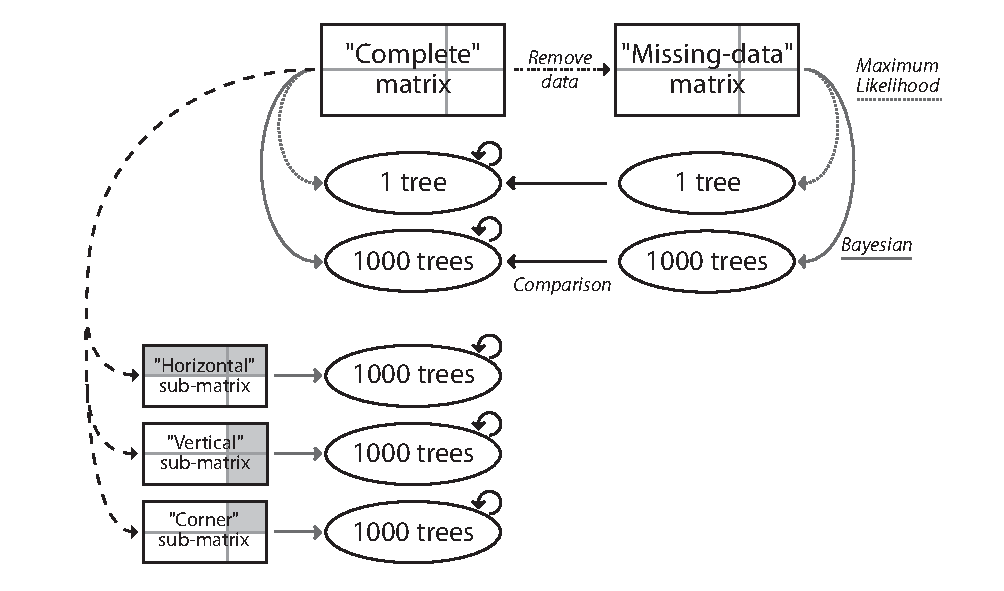
\includegraphics[keepaspectratio=true]{Figures/TEM_Fig_TreeCmp-BW.pdf}
%\caption{Tree comparison protocol.
%From each of the 125 parameters combination ($M_L$, $M_F$ and $M_C$), we inferred a tree in Baysian or Maximum likelihood framework. We then compared this tree with or without fossil/living taxa to the "best" tree.In the Bayesian framework, 1000 trees from the posterior distribution where used for each comparison.}
%\label{Fig_Compare}
%\end{figure}

%\subsubsection{Statistical difference between tree topologies} %note that in the end, I only have non-parametric tests, the parametric explanation part can go to the supplementaries
%To assess the difference between the tree topologies, whether they were inferred in a Bayesian or a ML framework, we performed a group comparison test for each set of configurations (e.g. effect of $M_L$ in Bayesian inference, combined effect of $M_F$ and $M_C$ in ML inference, etc...). We used the pairwise tree comparisons as factors (i.e. the "Best" tree vs. one of each of the 125 "missing-data" trees) and the values of the 51 replicates from the pairwise comparison as a response variable. The 51 replicates values were either the replicates of the 51 pairwise tree comparisons in ML or the modes of the 51 RPBTC posterior distributions in Bayesian. When we found a significant difference between the groups, we performed a pairwise comparison test to analyse which pairs of groups differ from the others. Depending on whether the data was normal with variance homoscedasticity or not (controlled by performing respectively a shapiro.test and a a bartlett.test in R\{stats\}), we used respectively parametric or non-parametric tests for the group comparison and the pairwise comparisons as suggested by \citet{ruxtontime2008} (Table ~\ref{Stats_test}). %link broken

%\begin{table}[ht]
%\caption{Statistical tests}
%\centering
%\begin{tabular}{lrll}
%  \hline
%   & test & statistics & code\{package\} \\ [0.5ex]
%  \hline
%  Groups comparisons & ANOVA & parametric & anova\{stats\} \\ [0.5ex]%
%                     & Kruskal-Wallis & non-parametric & kruskal.test\{%stats\} \\[0.5ex]
%  \hline
 % Pairwise comparisons & Tukey HSD & parametric & TukeyHSD\{stats\} \\ [0.5ex]
  %                     & Nemenyi-Damico-Wolfe-Dunn & non-parametric & kruskalmc\{pgirmess\} \\ [0.5ex]
 % \hline
%\end{tabular}
%\label{Stats_test}
%\end{table}

\subsection{Effect of missing molecular characters for fossil taxa} %Awful name.
% NC: Yeah!
% NC: OK you need to explain WHY we are doing this. What is this analysis designed to test. I think you said this was incomplete so I won't fix it I'll let you have a go first.
To assess the ability to recover topology for each simulation when no missing data was involved in the phylogenetic inference process, we split the "complete" matrix into three sub-matrices containing no missing data (see Fig. ~\ref{Fig_RemoveData}):
\begin{enumerate}
\item
A sub-matrix containing both molecular and morphological data for living taxa only;
%NC: Do you think the sub-matrix names are useful here? We won't use this as much as the "best" tree etc. So maybe just write it out each time? Also I don't like the names horizontal, vertical and corner - they don't really describe what is going on. Better something like - complete living, complete morphology, morphology living?
%TG: agreed.
\item
A sub-matrix containing morphological data for both living and fossil taxa;
\item
A sub-matrix containing morphological data for living taxa only ;
\end{enumerate}
We reran the Maximum Likelihood
%NC: Should we check ML trees too???
%TG: Not sure if it is necessary since this part (not fully developed yet) is yet another test to show that our results are significant and that the problem comes form the missing data in the fossils (or not???) 
and Bayesian tree inference and topology comparisons on the three sub-matrices in the same way as described above.


%---------------------------------------------
%       Empirical data - TO DO
%---------------------------------------------

\subsection{Empirical data} %Still not done!
Finally, to % NC: explain WHY we would want to do this
%TG: need to better explain an RUN this part, I'll rewrite this part properly ones the runs are over.

We also compared the results obtained from simulated data to results from empirical data in \citet{ronquista2012}.
The matrix (this would be the "complete" matrix using our terminology) contains 67 living species plus one outgroup and 45 fossil species of Hymenoptera with 5097 molecular characters and 354 morphological characters.
Because only 66 of the 68 living species in the matrix had molecular data, we treated these 66 taxa as "living" taxa and the remaining 47 as "fossil" taxa. 

We removed data from the "complete" matrix in the same way as described in steps 2 and 3 above, resulting in 124 matrices with various amount of missing data.
We used the same settings as described above to infer Maximum Likelihood trees, but for the Bayesian inferences we did not use any priors except the starting tree.
This consisted of the topology of the 68 living species with the highest posterior probability from non-clock analysis performed in \citet{ronquista2012}.
Note that we did not perform any of the clock analyses described in \citet{ronquista2012} because we were only interested in the topology of the inferred trees and not the branch lengths.

% NC: Is there a step missing here? What did you do (or what will you do) with these trees? Will you compare them to each other? How will you compare them to the simulations?


%---------------------------------------------
%
%       RESULTS
%
%---------------------------------------------


\section{Results}

% NC: OK it's worth thinking about what you really need to include here. Remember the results are about the answers to your question. Not necessarily everything you did. This section can be really short, and probably should be quite short.

% NC: I may have misunderstood but I don't think you need this section at all, or the comparing topologies section you have planned. Just the actual results surely...

%\subsection{Building the trees}
%When generating the matrices using seqgen \citep{ranbaut1997seqgen} and rTraitDisc \citep{paradisape:2004} algorithms with low evolutionary rate parameter ($\alpha$ = 0.5) we successfully generated evolutionary histories.
%In Maximum Likelihood, support values ranged from 0 to 100 with a median of 38 ($1^st$ quartile = 14, $3^rd$ quartile = 72 - see \hyperref[supplementaries]{supplementaries}). % This is actually bad.
%The distribution of the phylogenetic signal across the different chains provided us a good spread of evolutionary scenarios: from well resolved phylogenies to poorly resolved ones.
%This allows us to test our simulations in a theoretical as well as practical framework (i.e. phylogenies with low support values are rarely published but are still common in early stages of projects). %REF??? - That's kind of my way to turn these bad results into something usable: even if some of our simulations are not realistic, it shows the effect of missing data in any scenario possible, not only in realistic cases.
%Also, one can advocate that this low topological resolution is actively due to the amount of missing data in the total evidence matrices since the sub-matrices (no missing data) analysis recovers way higher support value  . %This is something that I will had with the whole submatrices story. Basically, when you have all the fossil/molecular data missing, it's harder to build the tree, both in ML and in Bayesian. When you run the analysis without missing data, then it works way better (i.e. our REAL control test: can we simulate matrices in the first place).
%Using Bayesian inference, all the chains converged with a significant effective sample size by using 2 parallel runs of 4 chains each (ASSD $<$ 0.01 and ESS $>>$ 200 for inference).

%\subsection{Comparing topologies}
%Did it worked? See sub-matrices part. TO DO

%\subsection{Effect of the missing data parameters}
% NC: Probably don't need a subheading here


\begin{figure} 
\centering
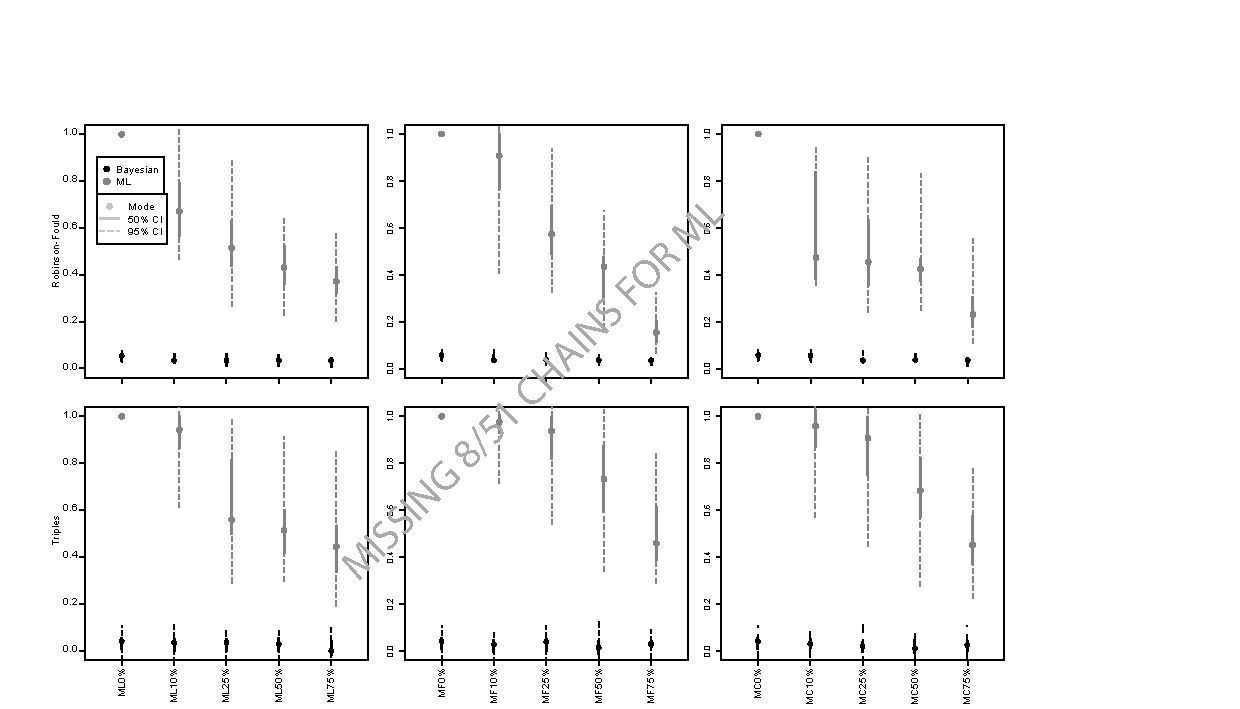
\includegraphics[keepaspectratio=true]{Figures/TEM_Fig-results-BW.pdf}
\caption{Effect of missing data on Tree similarity.
$M_L$ is the percentage of living taxa with no morphological data,
$M_F$ is the percentage of missing data in the fossil record,
$M_C$ is the percentage of missing morphological characters.
The first row represent the Normalized Tree Similarity index using the Robinson-Foulds metric;
the second row represent the Normalized Tree Similarity index using the Triples metric.}
\label{Fig_Results}
\end{figure}

%NC: OK from this point on you start referring to "Tree Similarity Index". This is not mentioned in the methods. What is it? You need to explain in the methods please.
%TG: stopped here 26/06.

%NC: I'm not sure you need to separate these three parameters out. Aren't you repeating yourself a lot? Rewrite this with them all in together. You can talk about general patterns and then specific, interesting patterns. I've corrected the first one a bit to help out.
\subsection{Effect of $M_L$}
In our Maximum Likelihood analyses, topological recovery (i.e. tree similarity) decreased as the percentage of missing data increased, using both the Triples and Robinson-Foulds metrics (see Table ~\ref{Group_results} - Fig.~\ref{Fig_Results}).
However, topological recovery was not significantly different for trees with 25\%, 50\% and 75\% missing morphological data for living taxa (Fig 1b???), % is this what you meant? And indicate the particular panel of the figure it refers to
suggesting that although tree topology is sensitive to this missing data, once it is greater than 25\% it makes little difference. Overall, the Robinson-Foulds metric shows lower tree similarities than the Triples metric. This indicates that the positions of individual taxa are generally more conserved than the membership of entire clades (see Table ~\ref{NTS_ML_results}).

Topological recovery was poor in our Bayesian analyses, regardless of the amount of missing data (Figures???), although topological recovery did decrease slightly as missing data increased. Overall, tree similarity index was only slightly above zero which means that trees are only slightly more similar than we would expect if we compared two completely random trees (see Table ~\ref{NTS_Ba_results}). 
%For the Triples metric there is no significant effect of the $M_L$ parameter, in other words, if living taxa are removed, there is no effect on the placement of "flying" taxa.
%For the Robinson-Fould metric, there is a significant effect of the $M_L$ leading small decrease in topological recovery when $M_L$ increases (see Table ~\ref{Ba_RF-ML_results}).

%NC: A shorter verison of this encompassing all three parameters will work here.

%NC: Combine with section above
\subsubsection{Effect of $M_F$}
In Maximum Likelihood framework, the effect of missing data in the fossil record appeared to be constant and led to a constant decrease in topological recovery when the missing data increased (see Table ~\ref{Group_results} - Fig. ~\ref{Fig_Results}).
The difference between the two metrics used is more important than for the $M_L$ parameter: clades are less conserved than individual taxa placement as the amount of missing data increases.
Interestingly, 10\% or 25\% missing data for the $M_F$ parameter does not seems to affect the apparition of unstable taxa (Triples NTS modes of respectively 0.97 and 0.93 - Table ~\ref{NTS_ML_results}).

Similarly than for the effect of $M_L$, Bayesian tree recovery was only slightly better than expected by chance.
In the same way as described above, there seems to be a small difference depending on the metric used.
There is no significant effect of the $M_F$ parameter when using the Triplet metric but the effect is significant when using the Robinson-Fould metric (see Table ~\ref{Ba_RF-MF_results}).
However, as mentioned previously the effect of the parameter $M_F$ is still minimal in a Bayesian framework (see Table ~\ref{Group_results} - Fig. ~\ref{Fig_Results}).

%NC: Combine with section above
\subsubsection{Effect of $M_C$}
The number of missing morphological characters ($M_C$), however, seems to be more affecting topological recovery than $M_L$ and $M_F$ (see Table ~\ref{Group_results} - Fig. ~\ref{Fig_Results}).
The Robinson-Fould metric shows a rapid drop in tree recovery from 10\% of missing data (Robinson-Fould NTS mode $<$ to 0.5 from 10\% missing data - Table ~\ref{NTS_ML_results}).
This decrease is however slower when using the Triples metric with still a good topological recovery at 10\%  (Triples NTS modes = 0.95 - Table ~\ref{NTS_ML_results}).

The effect of $M_C$ in Bayesian framework is similar as the one described for $M_L$ and $M_F$: tree recovery is only slightly better than expected by chance and only the Robinson-Fould metric shows a significant effect of the $M_C$ parameter on tree recovery (see Table ~\ref{Ba_RF-ML_results} and ~\ref{Group_results} - Fig. ~\ref{Fig_Results}).

%\subsubsection{Combined effect}
%Need to do the heat plots

$\newline$

%NC: This will be part of the section above. If it's short you may not need to sum up!
%To sum up:
%The ability of recovering the "best" tree's topology in Maximum Likelihood method is function of the amount of data missing.
%The parameters $M_C$ and $M_L$ have more influence than $M_F$ on decrease in topological recovery.
%The decrease in clade conservation (low Robinson-Fould NTS score) is faster than the increase in flying taxa (low Triples NTS score).
%In Bayesian framework, topology is badly (if not at all) recovered disregarding the amount of data missing.

% NC: You will need two sections here with subheadings - one for the sensitivity analyses you did with the submatrices, and one for the empirical results.


% NC: I would make these tables wider - so have a column for Triples, and one for RF, rather than a column for metric. same with Bayesian vs ML, why not have a set of columns instead? It'll take up less space and be easier to read I think...

% NC: You should do what I have done on the thesis template and have these tables as separate files rather than having them in the document.

% NC: we need to sit down and look at these tables. I don't like the current format.

% About the tables:

% What about making this table in a longevity-results style? with every thing combined (30 columns)?
% NC: That might be too many columns!

\begin{table}
  \centering
  \linespread{1.0}
  \caption{Tree similarity values per parameter in ML framework}
  \begin{tabular}{rrlccccc}
    \hline
    Parameter & amount of    & metric & mode & 50\%CI &       & 95\%CI &       \\
              & missing data &        &      & lower  & upper & lower  & upper \\
    \hline
    $M_L$     & 0\%          & Robinson-Fould & 1 & NA  & NA & NA  & NA \\
              &              & Triples        & 1 & NA  & NA & NA  & NA \\
              & 10\%         & Robinson-Fould & 0.669 & 0.588  & 0.815 & 0.397  & 1.057 \\ %
              &              & Triples        & 0.947 & 0.885  & 1.000 & 0.589  & 1.078 \\ %
              & 25\%         & Robinson-Fould & 0.506 & 0.421  & 0.627 & 0.280  & 0.867 \\ %
              &              & Triples        & 0.559 & 0.483  & 0.839 & 0.353  & 0.999 \\ %
              & 50\%         & Robinson-Fould & 0.427 & 0.360  & 0.507 & 0.188  & 0.660 \\ %
              &              & Triples        & 0.514 & 0.419  & 0.599 & 0.293  & 0.910 \\ %
              & 75\%         & Robinson-Fould & 0.363 & 0.302  & 0.428 & 0.184  & 0.543 \\ %
              &              & Triples        & 0.454 & 0.315  & 0.541 & 0.165  & 0.844 \\ %
    $M_L$     & 0\%          & Robinson-Fould & 1 & NA  & NA & NA  & NA \\
              &              & Triples        & 1 & NA  & NA & NA  & NA \\
              & 10\%         & Robinson-Fould & 0.893 & 0.723  & 0.985 & 0.384  & 1.031 \\ %
              &              & Triples        & 0.972 & 0.927  & 1.001 & 0.424  & 1.106 \\ %
              & 25\%         & Robinson-Fould & 0.559 & 0.482  & 0.692 & 0.220  & 0.951 \\ %
              &              & Triples        & 0.919 & 0.800  & 0.994 & 0.499  & 1.089 \\ %
              & 50\%         & Robinson-Fould & 0.436 & 0.302  & 0.476 & 0.140  & 0.668 \\ %
              &              & Triples        & 0.710 & 0.562  & 0.831 & 0.348  & 0.986 \\ %
              & 75\%         & Robinson-Fould & 0.139 & 0.097  & 0.193 & 0.055  & 0.323 \\ %
              &              & Triples        & 0.480 & 0.375  & 0.598 & 0.240  & 0.867 \\ %
    $M_L$     & 0\%          & Robinson-Fould & 1 & NA  & NA & NA  & NA \\
              &              & Triples        & 1 & NA  & NA & NA  & NA \\
              & 10\%         & Robinson-Fould & 0.463 & 0.354  & 0.842 & 0.314  & 0.970 \\ %
              &              & Triples        & 0.956 & 0.841  & 1.036 & 0.532  & 1.079 \\ %
              & 25\%         & Robinson-Fould & 0.471 & 0.323  & 0.616 & 0.213  & 0.888 \\ %
              &              & Triples        & 0.923 & 0.790  & 1.001 & 0.425  & 1.066 \\ %
              & 50\%         & Robinson-Fould & 0.421 & 0.354  & 0.479 & 0.128  & 0.823 \\ %
              &              & Triples        & 0.678 & 0.526  & 0.820 & 0.248  & 0.998 \\ %
              & 75\%         & Robinson-Fould & 0.220 & 0.170  & 0.282 & 0.076  & 0.571 \\ %
              &              & Triples        & 0.453 & 0.388  & 0.550 & 0.187  & 0.726 \\ %
    \hline
\end{tabular}
  \label{tab:NTS_ML_results}
\end{table}

\begin{table}
  \centering
  \linespread{1.0}
  \caption{Tree similarity values per parameter in Bayesian framework}
  \begin{tabular}{rrlccccc}
    \hline
    Parameter & amount of    & mode & 50\%CI &       & 95\%CI & \\
              & missing data &      & lower  & upper & lower  & upper \\
    \hline
    $M_L$     & 0\%          & Robinson-Fould & 0.056 & 0.035  & 0.063 & 0.031   & 0.076 \\ %how many digits?
              &              & Triples        & 0.041 & 0.008  & 0.054 & -0.039  & 0.106 \\
              & 10\%         & Robinson-Fould & 0.035 & 0.035  & 0.035 & 0.028   & 0.061 \\
              &              & Triples        & 0.033 & 0.003  & 0.049 & -0.049  & 0.117 \\
              & 25\%         & Robinson-Fould & 0.035 & 0.035  & 0.035 & 0.015   & 0.061 \\
              &              & Triples        & 0.035 & 0.002  & 0.049 & -0.041  & 0.096 \\
              & 50\%         & Robinson-Fould & 0.035 & 0.035  & 0.035 & 0.015   & 0.056 \\
              &              & Triples        & 0.028 & 0.003  & 0.052 & -0.038  & 0.092 \\
              & 75\%         & Robinson-Fould & 0.035 & 0.035  & 0.035 & 0.010   & 0.043 \\
              &              & Triples        & -0.001 & -0.018 & 0.040 & -0.060 & 0.106 \\
    $M_L$     & 0\%          & Robinson-Fould & 0.056 & 0.035  & 0.063 & 0.031   & 0.076 \\
              &              & Triples        & 0.041 & 0.008  & 0.054 & -0.039  & 0.106 \\
              & 10\%         & Robinson-Fould & 0.035 & 0.031  & 0.056 & 0.027   & 0.076 \\
              &              & Triples        & 0.026 & 0.002  & 0.050 & -0.046  & 0.105 \\
              & 25\%         & Robinson-Fould & 0.035 & 0.035  & 0.035 & 0.0153  & 0.068 \\
              &              & Triples        & 0.038 & 0.002  & 0.050 & -0.046  & 0.105 \\
              & 50\%         & Robinson-Fould & 0.035 & 0.035  & 0.035 & 0.015   & 0.058 \\
              &              & Triples        & 0.014 & -0.011 & 0.039 & -0.038  & 0.124 \\
              & 75\%         & Robinson-Fould & 0.035 & 0.035  & 0.035 & 0.015   & 0.041 \\
              &              & Triples        & 0.029 & 0.019  & 0.042 & -0.030  & 0.089 \\   
    $M_L$     & 0\%          & Robinson-Fould & 0.056 & 0.035  & 0.063 & 0.031   & 0.076 \\
              &              & Triples        & 0.041 & 0.008  & 0.054 & -0.039  & 0.106 \\
              & 10\%         & Robinson-Fould & 0.056 & 0.035  & 0.059 & 0.0281  & 0.076 \\
              &              & Triples        & 0.030 & 0.011  & 0.048 & -0.024  & 0.094 \\
              & 25\%         & Robinson-Fould & 0.035 & 0.035  & 0.035 & 0.023   & 0.076 \\
              &              & Triples        & 0.020 & -0.001 & 0.037 & -0.060  & 0.109 \\
              & 50\%         & Robinson-Fould & 0.035 & 0.035  & 0.035 & 0.030   & 0.059 \\
              &              & Triples        & 0.010 & -0.005 & 0.045 & -0.036  & 0.104 \\
              & 75\%         & Robinson-Fould & 0.035 & 0.035  & 0.035 & 0.011   & 0.043 \\
              &              & Triples        & 0.024 & 0.001  & 0.042 & -0.037  & 0.104 \\
    \hline
\end{tabular}
  \label{NTS_BA_results}
\end{table}

\begin{table}
  \centering
  \linespread{1.0}
  \caption{Group difference per configuration set}
  \begin{tabular}{rllcccc}
    \hline
    set & metric & framework & parametric & $stats^1$ & df & p.value \\
    \hline
    $M_L$         & Robinson-Fould & ML       & no & 174.768  & 4   & \textbf{0.00} \\
                  &                & Bayesian & no & 65.62    & 4   & \textbf{0.00} \\ 
                  & Triples        & ML       & no & 163.664  & 4   & \textbf{0.00} \\
                  &                & Bayesian & no & 4.56     & 4   & 0.34          \\ 
    $M_F$         & Robinson-Fould & ML       & no & 204.964  & 4   & \textbf{0.00} \\
                  &                & Bayesian & no & 85.61    & 4   & \textbf{0.00} \\
                  & Triples        & ML       & no & 172.992  & 4   & \textbf{0.00} \\
                  &                & Bayesian & no & 3.01     & 4   & 0.56          \\
    $M_C$         & Robinson-Fould & ML       & no & 170.779  & 4   & \textbf{0.00} \\ 
                  &                & Bayesian & no & 64.23    & 4   & \textbf{0.00} \\
                  & Triples        & ML       & no & 159.856  & 4   & \textbf{0.00} \\
                  &                & Bayesian & no & 26.13    & 24  & 0.35          \\
    $M_L+M_F$     & Robinson-Fould & ML       & no & 821.986  & 24  & \textbf{0.00} \\
                  &                & Bayesian & no & 317.97   & 24  & \textbf{0.00} \\
                  & Triples        & ML       & no & 586.873  & 24  & \textbf{0.00} \\
                  &                & Bayesian & no & 3.01     & 24  & 0.56          \\
    $M_L+M_C$     & Robinson-Fould & ML       & no & 601.293  & 24  & \textbf{0.00} \\
                  &                & Bayesian & no & 290.10   & 24  & \textbf{0.00} \\
                  & Triples        & ML       & no & 484.986  & 24  & \textbf{0.00} \\
                  &                & Bayesian & no & 22.19    & 24  & 0.57          \\
    $M_F+M_C$     & Robinson-Fould & ML       & no & 893.941  & 24  & \textbf{0.00} \\ 
                  &                & Bayesian & no & 385.96   & 24  & \textbf{0.00} \\
                  & Triples        & ML       & no & 596.049  & 24  & \textbf{0.00} \\
                  &                & Bayesian & no & 20.23    & 24  & 0.68          \\ 
    $M_L+M_F+M_C$ & Robinson-Fould & ML       & no & 3956.956 & 124 & \textbf{0.00} \\
                  &                & Bayesian & no & 1167.40  & 124 & \textbf{0.00} \\
                  & Triples        & ML       & no & 2260.953 & 124 & \textbf{0.00} \\
                  &                & Bayesian & no & 115.86   & 124 & 0.69          \\
    \hline
\end{tabular}

$^1$ F-value for parametric tests and Kruskal Wallis $chi^2$ for non parametric tests.
  \label{Group_results}
  $^1$ F-value for parametric tests and Kruskal Wallis $chi^2$ for non parametric tests.
\end{table}

\begin{table}
  \centering
  \linespread{1.0}
  \caption{$M_L$ non-parametric pairwise difference for Robinson-Fould metric in ML framework} 
  \begin{tabular}{c|ccccc}
    \hline
              & $M_L$00\% & $M_L$10\% & $M_L$25\% & $M_L$50\% & $M_L$75\% \\
    \hline
    $M_L$00\% & - & \textbf{TRUE}  & \textbf{TRUE} & \textbf{TRUE} & \textbf{TRUE}\\
    $M_L$10\% & & - & \textbf{TRUE}  & \textbf{TRUE} & \textbf{TRUE} \\
    $M_L$25\% & & & - & FALSE  & \textbf{TRUE} \\
    $M_L$50\% & & & & - & FALSE  \\
    $M_L$75\% & & & & & - \\
    \hline
\end{tabular}
\centering
\begin{tabular}{rrrl}
 pairwise comparison & obs.dif & critical.dif & difference \\ 
  \hline
  $M_L$00\%-$M_L$10\% & 56.53 & 37.66 & TRUE \\ 
  $M_L$00\%-$M_L$25\% & 96.85 & 37.66 & TRUE \\ 
  $M_L$00\%-$M_L$50\% & 127.03 & 37.66 & TRUE \\ 
  $M_L$00\%-$M_L$75\% & 144.58 & 37.66 & TRUE \\ 
  $M_L$10\%-$M_L$25\% & 40.31 & 37.66 & TRUE \\ 
  $M_L$10\%-$M_L$50\% & 70.50 & 37.66 & TRUE \\ 
  $M_L$10\%-$M_L$75\% & 88.05 & 37.66 & TRUE \\ 
  $M_L$25\%-$M_L$50\% & 30.19 & 37.66 & FALSE \\ 
  $M_L$25\%-$M_L$75\% & 47.73 & 37.66 & TRUE \\ 
  $M_L$50\%-$M_L$75\% & 17.55 & 37.66 & FALSE \\ 
   \hline
\end{tabular}
  \label{ML_RF-ML_results}
\end{table}

\begin{table}
  \centering
  \linespread{1.0}
  \caption{$M_L$ non-parametric pairwise difference for Triples metric in ML framework} 
  \begin{tabular}{c|ccccc}
    \hline
              & $M_L$00\% & $M_L$10\% & $M_L$25\% & $M_L$50\% & $M_L$75\% \\
    \hline
    $M_L$00\% & - & \textbf{TRUE}  & \textbf{TRUE} & \textbf{TRUE} & \textbf{TRUE}\\
    $M_L$10\% & & - & \textbf{TRUE}  & \textbf{TRUE} & \textbf{TRUE} \\
    $M_L$25\% & & & - & FALSE  & \textbf{TRUE} \\
    $M_L$50\% & & & & - & FALSE  \\
    $M_L$75\% & & & & & - \\
    \hline
\end{tabular}
\centering
\begin{tabular}{rrrl}
 pairwise comparison & obs.dif & critical.dif & difference \\ 
  \hline
  $M_L$00\%-$M_L$10\% & 72.14 & 40.60 & TRUE \\
  $M_L$00\%-$M_L$25\% & 119.30 & 40.60 & TRUE \\
  $M_L$00\%-$M_L$50\% & 136.67 & 40.60 & TRUE \\
  $M_L$00\%-$M_L$75\% & 166.89 & 40.60 & TRUE \\ 
  $M_L$10\%-$M_L$25\% & 47.16 & 40.60 & TRUE \\ 
  $M_L$10\%-$M_L$50\% & 64.53 & 40.60 & TRUE \\ 
  $M_L$10\%-$M_L$75\% & 94.75 & 40.60 & TRUE \\ 
  $M_L$25\%-$M_L$50\% & 17.37 & 40.60 & FALSE \\
  $M_L$25\%-$M_L$75\% & 47.59 & 40.60 & TRUE \\ 
  $M_L$50\%-$M_L$75\% & 30.22 & 40.60 & FALSE \\
   \hline
\end{tabular}
  \label{ML_Tr-ML_results}
\end{table}

\begin{table}
  \centering
  \linespread{1.0}
  \caption{$M_L$ non-parametric pairwise difference for Robinson-Foulds metric in Bayesian framework}
  \begin{tabular}{c|ccccc}
    \hline
              & $M_L$00\% & $M_L$10\% & $M_L$25\% & $M_L$50\% & $M_L$75\% \\
    \hline
    $M_L$00\% & - & FALSE & \textbf{TRUE} & \textbf{TRUE} & \textbf{TRUE}\\
    $M_L$10\% & & - & FALSE & \textbf{TRUE} & \textbf{TRUE} \\
    $M_L$25\% & & & - & FALSE & \textbf{TRUE} \\
    $M_L$50\% & & & & - & FALSE \\
    $M_L$75\% & & & & & - \\
    \hline
\end{tabular}
\centering
\begin{tabular}{rrrl}
 pairwise comparison & obs.dif & critical.dif & difference \\ 
  \hline
  $M_L$00\%-$M_L$10\% & 17.05 & 41.00 & FALSE \\ 
  $M_L$00\%-$M_L$25\% & 43.79 & 41.00 & TRUE \\ 
  $M_L$00\%-$M_L$50\% & 77.32 & 41.00 & TRUE \\ 
  $M_L$00\%-$M_L$75\% & 103.99 & 41.00 & TRUE \\ 
  $M_L$10\%-$M_L$25\% & 26.75 & 41.00 & FALSE \\ 
  $M_L$10\%-$M_L$50\% & 60.27 & 41.00 & TRUE \\ 
  $M_L$10\%-$M_L$75\% & 86.94 & 41.00 & TRUE \\ 
  $M_L$25\%-$M_L$50\% & 33.53 & 41.00 & FALSE \\ 
  $M_L$25\%-$M_L$75\% & 60.20 & 41.00 & TRUE \\ 
  $M_L$50\%-$M_L$75\% & 26.67 & 41.00 & FALSE \\ 
   \hline
\end{tabular}
  \label{Ba_RF-ML_results}
\end{table}

\begin{table}
  \centering
  \linespread{1.0}
  \caption{$M_F$ non-parametric pairwise difference for Robinson-Foulds metric in ML framework} 
  \begin{tabular}{c|ccccc}
    \hline
              & $M_F$00\% & $M_F$10\% & $M_F$25\% & $M_F$50\% & $M_F$75\% \\
    \hline
    $M_L$00\% & - & \textbf{TRUE} & \textbf{TRUE} & \textbf{TRUE} & \textbf{TRUE}\\
    $M_L$10\% & & - & FALSE & \textbf{TRUE} & \textbf{TRUE} \\
    $M_L$25\% & & & - & \textbf{TRUE} & \textbf{TRUE} \\
    $M_L$50\% & & & & - & \textbf{TRUE} \\
    $M_L$75\% & & & & & - \\
    \hline
\end{tabular}
\centering
\begin{tabular}{rrrl}
 pairwise comparison & obs.dif & critical.dif & difference \\ 
  \hline
  $M_F$00\%-$M_F$10\% & 59.27 & 37.66 & TRUE \\ 
  $M_F$00\%-$M_F$25\% & 79.72 & 37.66 & TRUE \\ 
  $M_F$00\%-$M_F$50\% & 120.70 & 37.66 & TRUE \\ 
  $M_F$00\%-$M_F$75\% & 167.81 & 37.66 & TRUE \\ 
  $M_F$10\%-$M_F$25\% & 20.45 & 37.66 & FALSE \\ 
  $M_F$10\%-$M_F$50\% & 61.43 & 37.66 & TRUE \\ 
  $M_F$10\%-$M_F$75\% & 108.55 & 37.66 & TRUE \\ 
  $M_F$25\%-$M_F$50\% & 40.98 & 37.66 & TRUE \\ 
  $M_F$25\%-$M_F$75\% & 88.09 & 37.66 & TRUE \\ 
  $M_F$50\%-$M_F$75\% & 47.12 & 37.66 & TRUE \\ 
   \hline
\end{tabular}
  \label{ML_RF-MF_results}
\end{table}

\begin{table}
  \centering
  \linespread{1.0}
  \caption{$M_F$ non-parametric pairwise difference for Triples metric in ML framework} 
  \begin{tabular}{c|ccccc}
    \hline
              & $M_L$00\% & $M_L$10\% & $M_L$25\% & $M_L$50\% & $M_L$75\% \\
    \hline
    $M_L$00\% & - & \textbf{TRUE} & \textbf{TRUE} & \textbf{TRUE} & \textbf{TRUE}\\
    $M_L$10\% & & - & FALSE & \textbf{TRUE} & \textbf{TRUE} \\
    $M_L$25\% & & & - & FALSE & \textbf{TRUE} \\
    $M_L$50\% & & & & - & FALSE \\
    $M_L$75\% & & & & & - \\
    \hline
\end{tabular}
\centering
\begin{tabular}{rrrl}
 pairwise comparison & obs.dif & critical.dif & difference \\
  \hline
  $M_L$00\%-$M_L$10\% & 77.35 & 40.60 & TRUE \\ 
  $M_L$00\%-$M_L$25\% & 102.49 & 40.60 & TRUE \\ 
  $M_L$00\%-$M_L$50\% & 143.04 & 40.60 & TRUE \\ 
  $M_L$00\%-$M_L$75\% & 174.62 & 40.60 & TRUE \\
  $M_L$10\%-$M_L$25\% & 25.14 & 40.60 & FALSE \\
  $M_L$10\%-$M_L$50\% & 65.69 & 40.60 & TRUE \\ 
  $M_L$10\%-$M_L$75\% & 97.27 & 40.60 & TRUE \\ 
  $M_L$25\%-$M_L$50\% & 40.55 & 40.60 & FALSE \\ 
  $M_L$25\%-$M_L$75\% & 72.13 & 40.60 & TRUE \\
  $M_L$50\%-$M_L$75\% & 31.58 & 40.60 & FALSE \\ 
   \hline
\end{tabular}
  \label{ML_Tr-MF_results}
\end{table}

\begin{table}
  \centering
  \linespread{1.0}
  \caption{$M_F$ non-parametric pairwise difference for Robinson-Fould metric in Bayesian framework}
  \begin{tabular}{c|ccccc}
    \hline
              & $M_F$00\% & $M_F$10\% & $M_F$25\% & $M_F$50\% & $M_F$75\% \\
    \hline
    $M_L$00\% & - & \textbf{TRUE} & \textbf{TRUE} & \textbf{TRUE} & \textbf{TRUE}\\
    $M_L$10\% & & - & FALSE & \textbf{TRUE} & \textbf{TRUE} \\
    $M_L$25\% & & & - & FALSE & \textbf{TRUE} \\
    $M_L$50\% & & & & - & FALSE \\
    $M_L$75\% & & & & & - \\
    \hline
\end{tabular}
\centering
\begin{tabular}{rrrl}
 pairwise comparison & obs.dif & critical.dif & difference \\ 
  \hline
  $M_F$00\%-$M_F$10\% & 64.78 & 37.66 & TRUE \\ 
  $M_F$00\%-$M_F$25\% & 89.09 & 37.66 & TRUE \\ 
  $M_F$00\%-$M_F$50\% & 123.20 & 37.66 & TRUE \\ 
  $M_F$00\%-$M_F$75\% & 150.43 & 37.66 & TRUE \\ 
  $M_F$10\%-$M_F$25\% & 24.31 & 37.66 & FALSE \\ 
  $M_F$10\%-$M_F$50\% & 58.42 & 37.66 & TRUE \\ 
  $M_F$10\%-$M_F$75\% & 85.65 & 37.66 & TRUE \\ 
  $M_F$25\%-$M_F$50\% & 34.10 & 37.66 & FALSE \\ 
  $M_F$25\%-$M_F$75\% & 61.34 & 37.66 & TRUE \\ 
  $M_F$50\%-$M_F$75\% & 27.23 & 37.66 & FALSE \\ 
   \hline
\end{tabular}
  \label{Ba_RF-MF_results}
\end{table}

\begin{table}
  \centering
  \linespread{1.0}
  \caption{$M_C$ non-parametric pairwise difference for Robinson-Fould metric in ML framework} 
  \begin{tabular}{c|ccccc}
    \hline
              & $M_C$00\% & $M_C$10\% & $M_C$25\% & $M_C$50\% & $M_C$75\% \\
    \hline
    $M_C$00\% & - & \textbf{TRUE} & \textbf{TRUE} & \textbf{TRUE} & \textbf{TRUE}\\
    $M_C$10\% & & - & FALSE & \textbf{TRUE} & \textbf{TRUE} \\
    $M_C$25\% & & & - & FALSE & \textbf{TRUE} \\
    $M_C$50\% & & & & - & \textbf{TRUE} \\
    $M_C$75\% & & & & & - \\
    \hline
\end{tabular}
\centering
\begin{tabular}{rrrl}
 pairwise comparison & obs.dif & critical.dif & difference \\ 
  \hline
  $M_C$00\%-$M_C$10\% & 67.99 & 37.66 & TRUE \\ 
  $M_C$00\%-$M_C$25\% & 87.58 & 37.66 & TRUE \\ 
  $M_C$00\%-$M_C$50\% & 116.16 & 37.66 & TRUE \\ 
  $M_C$00\%-$M_C$75\% & 155.77 & 37.66 & TRUE \\ 
  $M_C$10\%-$M_C$25\% & 19.59 & 37.66 & FALSE \\ 
  $M_C$10\%-$M_C$50\% & 48.17 & 37.66 & TRUE \\ 
  $M_C$10\%-$M_C$75\% & 87.78 & 37.66 & TRUE \\ 
  $M_C$25\%-$M_C$50\% & 28.58 & 37.66 & FALSE \\ 
  $M_C$25\%-$M_C$75\% & 68.19 & 37.66 & TRUE \\ 
  $M_C$50\%-$M_C$75\% & 39.60 & 37.66 & TRUE \\ 
   \hline
\end{tabular}
  \label{ML_RF-MC_results}
\end{table}

\begin{table}
  \centering
  \linespread{1.0}
  \caption{$M_C$ non-parametric pairwise difference for Triples metric in ML framework} 
  \begin{tabular}{c|ccccc}
    \hline
              & $M_C$00\% & $M_C$10\% & $M_C$25\% & $M_C$50\% & $M_C$75\% \\
    \hline
    $M_C$00\% & - & \textbf{TRUE} & \textbf{TRUE} & \textbf{TRUE} & \textbf{TRUE}\\
    $M_C$10\% & & - & FALSE & \textbf{TRUE} & \textbf{TRUE} \\
    $M_C$25\% & & & - & FALSE & \textbf{TRUE} \\
    $M_C$50\% & & & & - & FALSE \\
    $M_C$75\% & & & & & - \\
    \hline
\end{tabular}
\centering
\begin{tabular}{rrrl}
 pairwise comparison & obs.dif & critical.dif & difference \\ 
  \hline
  $M_C$00\%-$M_C$10\% & 88.21 & 40.60 & TRUE \\ 
  $M_C$00\%-$M_C$25\% & 102.79 & 40.60 & TRUE \\ 
  $M_C$00\%-$M_C$50\% & 133.76 & 40.60 & TRUE \\ 
  $M_C$00\%-$M_C$75\% & 172.74 & 40.60 & TRUE \\ 
  $M_C$10\%-$M_C$25\% & 14.58 & 40.60 & FALSE \\ 
  $M_C$10\%-$M_C$50\% & 45.55 & 40.60 & TRUE \\
  $M_C$10\%-$M_C$75\% & 84.53 & 40.60 & TRUE \\ 
  $M_C$25\%-$M_C$50\% & 30.97 & 40.60 & FALSE \\ 
  $M_C$25\%-$M_C$75\% & 69.95 & 40.60 & TRUE \\ 
  $M_C$50\%-$M_C$75\% & 38.98 & 40.60 & FALSE \\ 
   \hline
\end{tabular}
  \label{ML_Tr-MC_results}
\end{table}

\begin{table}
  \centering
  \linespread{1.0}
  \caption{$M_C$ non-parametric pairwise difference for Robinson-Fould metric in Bayesian framework}
  \begin{tabular}{c|ccccc}
    \hline
              & $M_C$00\% & $M_C$10\% & $M_C$25\% & $M_C$50\% & $M_C$75\% \\
    \hline
    $M_C$00\% & - & FALSE & FALSE & \textbf{TRUE} & \textbf{TRUE}\\
    $M_C$10\% & & - & FALSE & \textbf{TRUE} & \textbf{TRUE} \\
    $M_C$25\% & & & - & FALSE & \textbf{TRUE} \\
    $M_C$50\% & & & & - & FALSE \\
    $M_C$75\% & & & & & - \\
    \hline
\end{tabular}
\centering
\begin{tabular}{rrrl}
 pairwise comparison & obs.dif & critical.dif & difference \\ 
  \hline
  $M_C$00\%-$M_C$10\% & 16.03 & 41.00 & FALSE \\ 
  $M_C$00\%-$M_C$25\% & 38.50 & 41.00 & FALSE \\ 
  $M_C$00\%-$M_C$50\% & 61.52 & 41.00 & TRUE \\ 
  $M_C$00\%-$M_C$75\% & 95.52 & 41.00 & TRUE \\ 
  $M_C$10\%-$M_C$25\% & 22.47 & 41.00 & FALSE \\ 
  $M_C$10\%-$M_C$50\% & 45.49 & 41.00 & TRUE \\ 
  $M_C$10\%-$M_C$75\% & 79.49 & 41.00 & TRUE \\ 
  $M_C$25\%-$M_C$50\% & 23.02 & 41.00 & FALSE \\ 
  $M_C$25\%-$M_C$75\% & 57.02 & 41.00 & TRUE \\ 
  $M_C$50\%-$M_C$75\% & 34.00 & 41.00 & FALSE \\ 
   \hline
\end{tabular}
  \label{Ba_RF-MC_results}
\end{table}

%---------------------------------------------
%
%       DISCUSSION
%
%---------------------------------------------

\section{Discussion}

% NC: Discussions usually begin with a paragraph that sums up the results. Then you can move on to discussing caveats, problems, extentions etc. You also need to show how your work fits in with the wider literature. So I think you need to re-write this completely with that in mind. Do the same as we did for the introduction - write a line for each paragraph. This reads like you jumped in without thinking clearly about the structure. It probably doesn't need to have all the same subheadings either.

\subsection{Building the trees}
Simulating evolutionary history matrices still remains a big drawback in theoretical phylogenetics. %Hahahaha.... feck.
The size of our simulated matrices was at least two orders orders of magnitude lower than usual matrices, both for the molecular part \citep[e.g.][]{springermacroevolutionary2012} and the morphological part \citep[e.g.][]{nithe2013}. % NC: Caveats later on
This configuration probably lead to globally low phylogenetic signal as well as the intrinsic difficulties to simulated characters with phylogenetic signal.
Even though molecular characters evolution (and therefore simulation) only depends of a small number of parameters (i.e. the base frequencies and the substitution matrix), simulating molecular matrix with a strong evolutionary signal is still complicated when generating unrealistically small matrices.
For morphological characters, the underlying pattern of their evolution are often more complex and ruled by more parameters than molecular characters (i.e the number of character states, the states frequencies, the substitution matrix and the statistical model used) \citep{Pagel22011994,wagner2000,lewisa2001}.

Also morphological characters studies involve many potential statistical pitfalls (e.g. independent characters violation, rate variation - \citet{davalosintegrating2014}) and especially (i) incongruence with molecular signal and (ii) homoplasy. %REF probably April has something about it
\begin{enumerate}
\item{First, morphological data can display a different signal than molecular data, especially in small matrices. %REF
This might lead to a controversial phylogenetic signal in the overall matrix and lower down the support values.
However, regarding empirical data studies, most of the groups shows fairly congruent morphological and molecular phylogenetic signal \citep[e.g.][]{leerates2013}.}
%The main difference between molecular and morphological characters is that, because of historical and practical reasons, a morphological character matrix do no contains autapomorphies and invariant characters which are usually more common than synampomorphies in molecular character matrices (cite).
\item{Secondly, in this study, we made the assumption that theoretically, morphological characters are randomly distributed on an organism however it seems clear that empirical morphological data does not act randomly \citep{sansomfossilization2013}.
However, following our simulation assumption of random character distributions, if they accumulate through time in the same way as the majority of the molecular characters then, homoplasic characters are expected to appear randomly through time \citep{davalosintegrating2014}.
Therefore, homoplasy is expected to be more important (by chance) in bigger morphological matrices \citep{davalosintegrating2014}.
After a reaching a critical amount of morphological characters, adding new ones increases homoplasy \citep{wagner2000}.}
\end{enumerate}
Our simulation parameters both decrease the phylogenetic signal (difficulty to simulate morphological characters and size of the matrix) as well as it increases it (reduction of homoplasy in the morphological part of the matrix).
Therefore, these drawbacks seems to have only a minor impact on the main results of this study: the incapacity of recovering any topology in Bayesian inference.

\subsection{Comparing topologies} % NC: Is any of this really relevant to the central questions of the paper? I don't think so... Maybe some of this could go in the methods where you chose these metrics. But it may not even be needed there.
Comparing topologies is a crucial question in phylogenetics but has always been hard to normalise because of the vast amount of different metrics used as proxies for different aspects of tree similarity/dissimilarity \citep{agapowpower2002}.
Because our global framework is to study how to include efficiently fossils into phylogenies, we chose metrics reflecting the most interesting aspect of this global question: where do individual taxa (i.e. the fossils) branch in the tree.
The Robinson-Foulds \citep{RF1981} and the Triples \citep{critchlowthe1996} metrics are more sensible to taxa and clade placement than other tree comparison metrics \citep[e.g.][Imbalance metric]{kirkpatricksearching1993} and where therefore favored.
Also by using the Normalized Tree Similarity index \citep{Bogdanowicz2012} we emphasize the aspect of "good" phylogenetic signal \textit{versus} random phylogenetic signal because it normalized the values of the metric by correcting for the expected value when comparing random trees (NTS = 0).

The Robinson-Fould metric is a conservative tree topology metric, it is more sensible to single taxon displacement because it will count clades as similar only if they are composed of the same number of taxa with the same topologies \citep{RF1981}.
When getting closer to the root of the tree, displacement of single taxon makes the clades not being exactly identical any more even if the clade still contains all the other taxa in both trees.
On the other hand, the Triples method is measuring the position of each taxon towards to other reference taxa \citep{critchlowthe1996}.
It will penalise only trees where taxa get removed furthest from their original clade.
Regarding our problematic (how does missing data influence topological recovery in trees containing both living and fossil taxa) we are more interested the placement of taxa (i.e. where does the fossil branch) than the exact conservation of clades.

%Need a transition!

Although the idea of comparing two single trees is straightforward, it becomes more complex when comparing trees distributions (e.g. Bayesian posterior distributions).
The introduction of our Random Pairwise Bayesian Tree Comparison methods allows to summarize the comparison of two trees distributions by picking up the most frequent signal in the distribution of the pairwise comparisons (i.e. the mode).
Even though this method is subject to randomness and might artificially increase or decrease the score of the studied metric, simulations showed that when a sufficient amount of random comparisons is performed, this method doesn't seem to be subject to randomness (e.g. 1000 random pairwise comparisons - see ~\ref{supplementaries}).

\subsection{Maximum Likelihood versus Bayesian}
The main results of our analysis shows that Bayesian inference fails to recover any Topology in a Total Evidence method framework (Fig. ~\ref{Fig_Results}).
This results is surprising regarding the behaviour of Maximum Likelihood inference (Fig. ~\ref{Fig_Results}) as well as the Bayesian inferences performed on empirical data \citep{ronquista2012,schragocombining2013}.
However, it is important to note that this effect was not mentioned in the aforementioned empirical tests because both studies used a Bayesian approach with fixed topology \citep{ronquista2012,schragocombining2013}.

In our case, we suspect that this inability of Bayesian methods to recover topology is due to the intrinsic structure of a Total Evidence matrix (Fig ~\ref{Fig_RemoveData}).
In fact, as previously studies have shown, missing data doesn't seem to be a major drawback as long as the missing data is randomly distributed ~\citep[e.g.][]{wiensmissing2003,rouresite-specific2011,sansomfossilization2013}.
However, in Total Evidence matrices, the majority of the missing data is not randomly distributed but concentrated in the molecular part of the matrix for the fossil taxa (i.e. the missing-data sub-matrix, Fig ~\ref{Fig_RemoveData}).
This leads to high decrease of topological recovery when using non optimal criterion approach (i.e. Bayesian inference) because of the high variance in the near-likeliest solutions sampled in the Bayesian posterior distribution.
In opposition, when applying optimal criterion approach (i.e. Maximum Likelihood), it is still possible to sample the likeliest tree. %probably need to develop that way more, especially with actually analysing the likelihood landscape.

\subsection{Effect of missing data}
The three parameters we selected in this study account for three potential pitfalls in collecting the data for Total Evidence analysis:
$M_L$ represents the living taxa for which there is no available morphological data,
$M_F$ represents the quality of the fossil record,
and $M_C$ represents the general coding effort and the overall of morphological data available.
Ideally, the lowest possible amount of missing data is wanted in any phylogenetic analysis leading to a data collection part prior to the phylogenetic analysis.
Each of the three parameters can be improved in a different way prior to the analysis:
for $M_L$, one should put more effort in using natural museums history collections for coding the missing morphological data for living taxa if possible %go to the museum!;
for the $M_F$ parameter, the amount of missing data unfortunately depends on the quality of the fossil record and can not be actively improved and depends on exceptional discoveries \citep[e.g.][]{nithe2013};
finally for the $M_C$ parameter, improvement can be done by vast collaborative projects in order to gather as much characters as possible \citep[e.g.][]{O'Leary08022013}.

Our results shows that the $M_F$ parameter have less influence on recovering the good tree topology in Maximum Likelihood framework which is fortunate since it is the parameter that is the more difficult to fix for practical reasons.
Regarding the fact that we are more interested in taxa placement than in clade conservation (Triples \textit{versus} Robinson-Fould), the parameter that affects the more the decrease in topological recovery is the number of missing living taxa in the morphological part of the matrix ($M_L$) and the overall number of morphological characters $M_C$.
This makes sense since the living taxa are bearing both the information to build the tree backbone (the molecular data) and the information used for branching the fossil on this backbone (the morphological information).
Therefore, we advocate the importance of coding morphological characters for the most living taxa possible and with the most characters possible, potentially by using collaborative projects portals such as morphobank \citep{morphobank}.  





%Potential reviewers comments?
%What about it when you vary the proportion of fossil taxa?


%---------------------------------------------
%
%       CONCLUSION
%
%---------------------------------------------


\section{Conclusion}
A Bayesian approach fails to recover accurate topology in a Total Evidence approach framework, whatever the amount of missing data.
We think this failure is due to the intrinsic structure of the Total Evidence matrices that includes a vast amount of non randomly distributed missing data (i.e. the molecular part of the matrix for the fossil taxa).
This missing data is equal to the number of fossil taxa $\times$ the number of molecular characters leading to a vast amount of trees to be sampled in Bayesian posterior distribution.
However, one can use a Maximum Likelihood approach to fix the likeliest topology.
If so, an effort should be made prior to the phylogenetic analysis on collecting as much morphological data as their is available from living taxa in order to efficiently improve the quality of the trees.

%Perspectives:
%What the effect of this missing molecular data on branch length estimation?

%---------------------------------------------
%
%       ...
%
%---------------------------------------------


\section{Acknowledgements}
% NC: Try and keep these short and to the point
Thanks to Fr\'{e}d\'{e}ric Delsuc, Emmanuel Douzery, Trevor Hodkinson and Andrew Jackson, Gavin Thomas, April Wright and the members of the Macro Journal Club %Also Gavin Thomas if not authors - %TG : also Adam Kev and Sive or that's putting to many people, thinking about it, they helped at least as much as Andrew (not mentioning Trevor but that's more political)?
for useful comments on our simulation protocol. Thanks to Paddy Doyle, Graziano D'Innocenzo and Sean McGrath for assistance with the computer cluster. Simulations used the Lonsdale cluster maintained by the Trinity Centre for High Performance Computing and funded through grants from Science Foundation Ireland. % NC: Is this what you're supposed to cite for the cluster? Check. - TG: yep
This work was funded by a European Commission CORDIS Seventh Framework Programme (FP7) Marie Curie CIG grant (proposal number: 321696).

%BIBLIOGRAPHY
 % The \cite command functions as follows:
 %   \citet{key} ==>>                Jones et al. (1990)
 %   \citet*{key} ==>>               Jones, Baker, and Smith (1990)
 %   \citep{key} ==>>                (Jones et al., 1990)
 %   \citep*{key} ==>>               (Jones, Baker, and Smith, 1990)
 %   \citep[chap. 2]{key} ==>>       (Jones et al., 1990, chap. 2)
 %   \citep[e.g.][]{key} ==>>        (e.g. Jones et al., 1990)
 %   \citep[e.g.][p. 32]{key} ==>>   (e.g. Jones et al., p. 32)
 %   \citeauthor{key} ==>>           Jones et al.
 %   \citeauthor*{key} ==>>          Jones, Baker, and Smith
 %   \citeyear{key} ==>>             1990

\bibliographystyle{sysbio} %don't write the suffix
\bibliography{References} %don't write the suffix

\section{Supplementary Material}
% NC: What do they call this in Syst Biol? Supplemental Materials is more usual...
% NC: You probably want to give these numbers so you can refer people to supp mat section 1, section 2 etc. etc.
    \documentclass[12pt,letterpaper]{article}

%Packages
\usepackage{pdflscape}
\usepackage{fixltx2e}
\usepackage{textcomp}
\usepackage{fullpage}
\usepackage{natbib}
\usepackage{float}
\usepackage{latexsym}
\usepackage{url}
\usepackage{epsfig}
\usepackage{graphicx}
\usepackage{amssymb}
\usepackage{amsmath}
\usepackage{bm}
\usepackage{array}
\usepackage[version=3]{mhchem}
\usepackage{ifthen}
\usepackage{caption}
\usepackage{hyperref}
\usepackage{amsthm}
\usepackage{amstext}
\usepackage{enumerate}
\usepackage[osf]{mathpazo}
\usepackage{dcolumn}
\usepackage{lineno}
\pagenumbering{arabic}


%Pagination style and stuff
\linespread{2}
\raggedright
\setlength{\parindent}{0.5in}
\setcounter{secnumdepth}{0} 
\renewcommand{\section}[1]{%
\bigskip
\begin{center}
\begin{Large}
\normalfont\scshape #1
\medskip
\end{Large}
\end{center}}
\renewcommand{\subsection}[1]{%
\bigskip
\begin{center}
\begin{large}
\normalfont\itshape #1
\end{large}
\end{center}}
\renewcommand{\subsubsection}[1]{%
\vspace{2ex}
\noindent
\textit{#1.}---}
\renewcommand{\tableofcontents}{}
\bibpunct{(}{)}{;}{a}{}{,}

\section{Code}
All code for performing the analyses is available at: \url{https://github.com/TGuillerme/Total_Evidence_Method-Missing_data}.

\newpage
\section{Appendix 1: Tree Building}
  \section{Supplementary material Section 1}

\subsection{Morphological characters states}
In order to obtain a realistic probabilistic value for of \textit{k} characters states for each simulated morphological character, we downloaded 100 random morphological characters (with more than 100 characters each) from TreeBASE database (http://treebase.org/) published between 1985 and 2013 and covering 19 taxomomic classess (Chordata, Arthropoda, Annelida, Angiosperm, Gymnosperm and Pteridophyta).
We selected a total of 22563 characters ranging from 2 to 10 states.
We calculated the proportion of characters with 2, 3, 4, 5, 6, 7, 8, 9 or 10 states.
We then sampeled 22563 \textit{k} values between 2 and 10 with the same proportion of characters from the empirical data.
We then used a simple t-test to check if our simulation was equal to the empirical data.
In this study, we only simulated characters with 2 or 3 states because of the high proportion of ordered characters ecountered on characters with more than 3 states and the difficulties of simulate biologicaly sensible ordered characters.

\begin{figure}
\centering
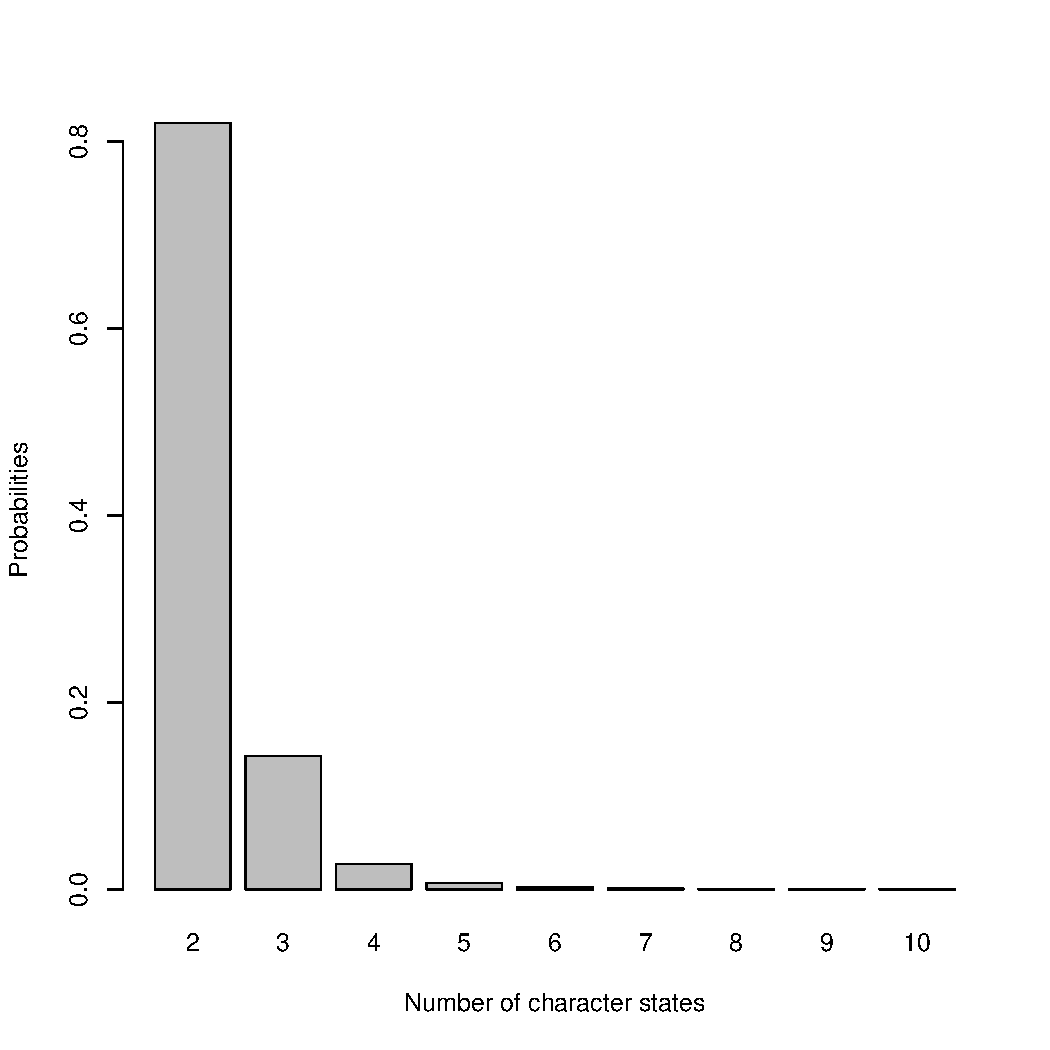
\includegraphics[keepaspectratio=true]{Figures/Supplementary/TEM_Fig-AppendixCharacters.pdf}
\caption{Character states distribution in empirical matrices. %Title?
Characters states number distribution extracted from 100 random morphological matrices downloaded from RreeBase.}
\label{Fig_AppendixCharacters}
\end{figure}


\subsection{Tree Building Software settings}

\subsubsection{Maximum Likelihood - RAxML v8.0.20 \citep{Stamatakis21012014}}

Model: \\
Molecular data: \\
GTR + $\Gamma_4$ (-m GTRGAMMA) \\
Morphological data: \\
Mk + $\Gamma_4$ (-K MK) \\
Support: \\
Rapid Boostrap algorithm (LSR), 1000 replicates \\

\subsubsection{Bayesian - MrBayes v3.2.1 \citep{Ronquist2012mrbayes}}

Priors: \\
Molecular data: \\
rates distribution shape ($\alpha$) = 0.5 \\
Transition/Transversion ratio = 2 ($\beta$(80,40)) \\
Starting tree: "True" tree topology with each branch length = 1 \\
Morphological data: \\
rates distribution shape ($\alpha$) = 0.5 \\
Models: \\
Molecular data: HKY + $\Gamma_4$ \\
Morphological data: Mk + $\Gamma_4$ \\
MCMC: \\
2 runs \\
4 chains per run \\
generations < 50$\times$$1^6$ \\
sample frequency = 1050$\times$$1^3$ \\
ASDS diagnosis frequency = 50$\times$$1^3$ \\
ASDS $<$ 0.01 \\
ESS $>>$ 200 \\
Burnin = 25\%
  \label{Supp_TreeBuilding}

\newpage
\section{Appendix 2: Tree Comparisons}
  %\section{Supplementary material Section 2}

\subsection{Robinson-Foulds distance}
Robinson-Foulds distance (\textit{RF}; \citealp{RF1981}), or "path difference", measures the number of shared clades across two trees. The metric reflects the distance between the distributions of tips among clades in the two trees \citep{RF1981} and can be expressed as:
\begin{equation}
RF_{x,y} = N_{x} + N_{y} - 2C_{x,y}
\end{equation}
where $C_{x,y}$ is the number of clades in common in the two trees. $C$ is equal to one if the two trees have the same $n$ taxa; and $C = n-2$ when none of the $n$ taxa are shared between the trees. This metric is more sensitive to taxon displacement than Triplets distance (i.e. if one taxon moves out of a clade, then the clades are no longer considered similar; \citet{critchlowthe1996,johnson1998,wiensmissing2003}). The minimal value of $C$ is equal to 1 if the two trees have the same n taxa; the maximal value in $C = n-2$. For a fully unresolved tree (star tree) $N$=1 and for a fully resolved tree (binary tree) $N = n-2$. The minimal and maximal topological distance for taxa is:
\begin{equation}
RF_{min} = 1 + 1 - 2C_{x,y}
\end{equation}
and:
\begin{equation}
RF_{max} = 2(n-2)-2
\end{equation}
One can then rescale \textit{RF.scaled} by using the maximal and minimal value for any $n$ taxa:
\begin{equation}
RF.scaled_{x,y} = \frac{RF_{x,y}-RF_{max}}{RF_{max}}
\end{equation}
This metric is more sensitive to taxa displacement than the Triplets distance \citep{critchlowthe1996,johnson1998,wiensmissing2003} and therefore a low value will show a good clade conservation between two trees and a high value will show a bad recovery of common clades.

\subsection{Triplets distance details ($T_{x,y}$)}
Triplets distance ($T_{x,y}$; \citealp{dobson1975triplets}) measures the number of sub-trees made up of three taxa (triplets) that differ between two given trees. Each triplet can be written as $I_{ijk}$=(\textit{ijk}). Where $I_{ijk}$ is equal to zero if the the two triplets (\textit{ijk}) are the same in the two trees otherwise $I_{ijk}$ is equal to one. For any rooted binary tree there are only three possible combinations for each triplet: ((\textit{j},\textit{k}),\textit{i});, ((\textit{i},\textit{k}),\textit{j}); and ((\textit{i},\textit{j}),\textit{k}); \citep{johnson1998}. If the trees used are not fully binary, a fourth triplet combination is possible: (\textit{i},\textit{j},\textit{k}). We can calculate the triplet distance between two trees, $S_n$, as:
\begin{equation}
S_n = \sum_{ijk} I_{ijk}
\end{equation}
where:
\begin{equation}
\sum_{ijk} = \binom{n}{4} = \frac{n!}{4!(n-4)!}
\end{equation}
and where \textit{n} is the total number of taxa in both trees (modified from \citet{critchlowthe1996}). If $S_n$ = 0, the trees are identical; when $S_n$ = $\binom{n}{4}$, the trees are as different as possible (i.e. every taxon has a different placement in the two trees). Because the possible number of triplets per clade is a finite number, the probability of two random trees with the same $n$ taxa to have the same triplet is:
\begin{equation}
P({I_{ijk}}=0) = \frac{1}{4}
\end{equation}
Therefore one can calculate the probability of two random trees having the same triplets: 
\begin{equation}
P({S_{n}}=0) = \sum_{ijk} P_{I_{ijk}=0}
\end{equation}
\begin{equation}
P({S_{n}}=0) = \frac{n!}{4(3!(n-3)!}
\end{equation}
and in the same way:
\begin{equation}
P({S_{n}}=1) = \frac{3n!}{4(3!(n-3)!}
\end{equation}

\subsection{Normalised Tree Similarity}
For any tree with \textit{n} taxa compared using a tree distance metric $m$, Normalized Tree Similarity, $NTS_m$ \citep{Bogdanowicz2012}, represents the similarity score for the two trees given the expected distance between two random Yule trees with $n$ taxa. If $\bar{d}_{m,n}$\textit{(rand)} is the average distance between two random Yule trees with $n$ taxa and $d_{m,n}$\textit{(x,y)} the distance between the two trees \textit{x} and \textit{y} each containing $n$ taxa, then:
\begin{equation}
NTS_{m,n}(x,y)=\frac{\bar{d}_{m,n}(rand) - d_{m,n}(x,y)} {\bar{d}_{m,n}(rand)}
\end{equation}
\textit{NTS} ranges from one to -$\infty$.
For any $m,n$, when $NTS$ = 1, the trees are identical, when \textit{NTS} = 0 the trees are no more different than expected by chance, and when $NTS$ $<$ 0, the trees are more different than expected when comparing two random trees. 

We used the NTS method to scale all the Robinson Foulds and Triplets distances calculated in our analyses, using the TreeCmp java script \citep{Bogdanowicz2012}.

\subsection{Bhattacharyya Coefficient}
The Bhattacharyya Coefficient calculates the probability of overlap of two distributions \citep{Bhattacharyya}. When it is equal to zero, the probability of overlap of the distributions is also zero, and when it is equal to one, the two distributions are entirely overlapping. It forms an elegant and easy to compute continuous measurement of the probability of similarity between two distributions. The coefficient is calculated as the sum of the square root of the relative counts shared in \textit{n} bins among two distributions.
\begin{equation}
\text{Bhattacharyya Coefficient}=\sum_{i=1}^{n} \sqrt{{\sum{a_i}}\times{\sum{b_i}}}
\end{equation}
where
\begin{equation}
\sum{a_i}=\frac{\text{Number of counts in bin \textit{i} for the distribution \textit{a}}}{\text{Total number of counts for the distribution \textit{a}}}
\end{equation}
and
\begin{equation}
\sum{b_i}=\frac{\text{Number of counts in bin \textit{i} for the distribution \textit{b}}}{\text{Total number of counts for the distribution \textit{b}}}
\end{equation}
The precision of the Bhattacharyya Coefficient is directly related to the number of bins, $n$. If $n$ is low, the overlap will be overestimated and if $n$ is too high, the overlap will be underestimated. In this analysis, we determined the number of bins using Silverman's rule of thumb which states that $n$ should be 0.9 times the minimum of the standard deviation and the interquartile range of the distribution, divided by 1.34 times the sample size of the distribution to the negative one-fifth power (bw.nrd0() function in R; \citet{silverman1986density}).

  \label{Supp_TreeComparison}

\bibliographystyle{sysbio}
\bibliography{Supp_Ref}

\newpage
\section{Appendix 3: Additional Results}
  \section{Supplementary material Section 3}

\begin{figure} 
\centering
    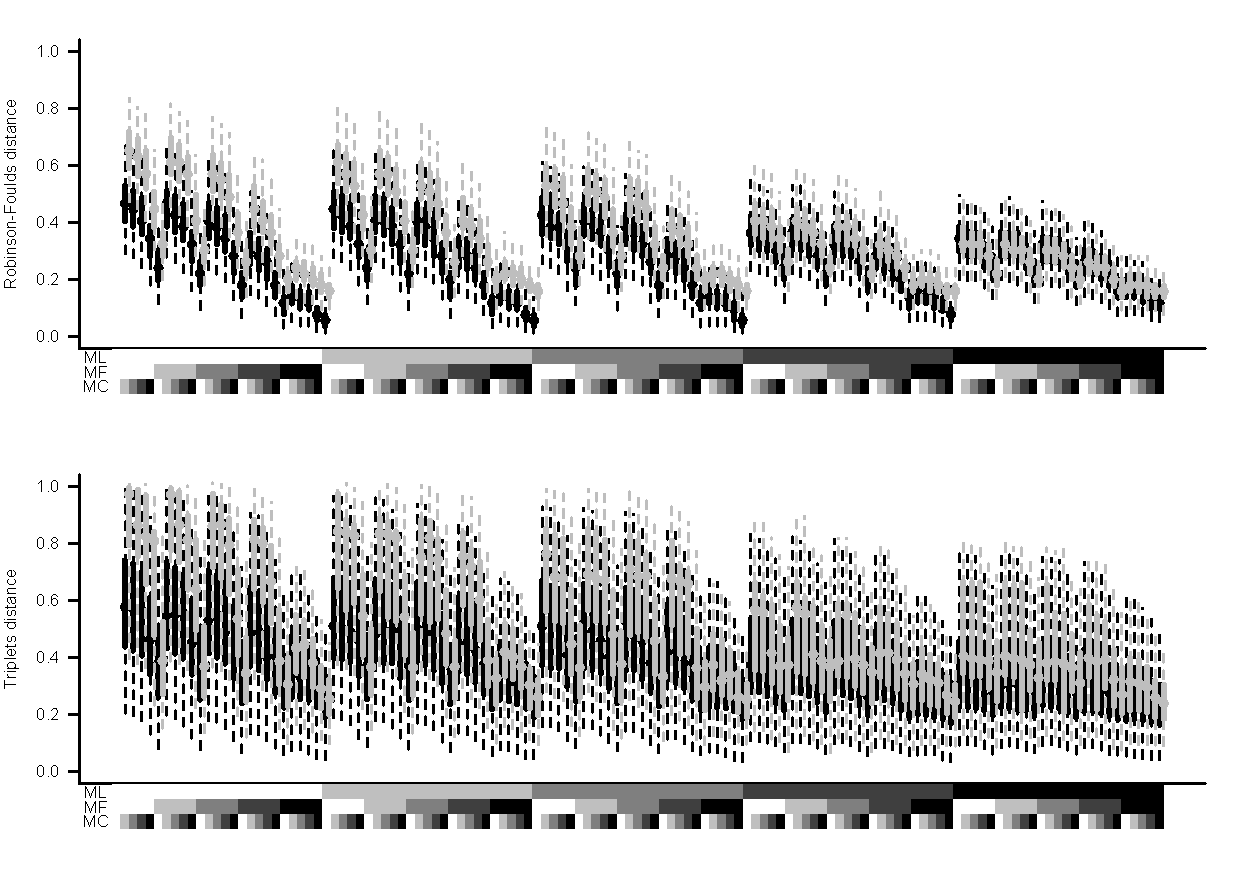
\includegraphics[width=1\textwidth]{SupplementaryMaterial/Supp_Figures/Boot+Baytre-AllParam-RF+Tr.pdf}
\caption{Trend of the effect of missing data on topological recovery on the Bootstraps and the Bayesian posterior trees distributions. The amount of missing data per parameter ($M_{L}$, $M_{F}$ and $M_{C}$) is represented along the x axis. The colour gradient from white to black represents respectively, 0\%, 10\%, 25\%, 50\% and 75\% of missing data. The topological recovery is represented on the y axis, both using Robinson-Foulds distance (upper row) and Triplets distance (lower row). Points represent the modal value of each distribution ; thick solid and thin dashed lines represents respectively the 50\% and 95\% confidence intervals or the distributions. The Bootstraps are represented in black and the Bayesian posterior trees distributions in grey.}
\label{Fig_global_BootTreesets} %Differences between all the parameters and between two methods (Boot vs treesets)
\end{figure}

\begin{figure} 
\centering
    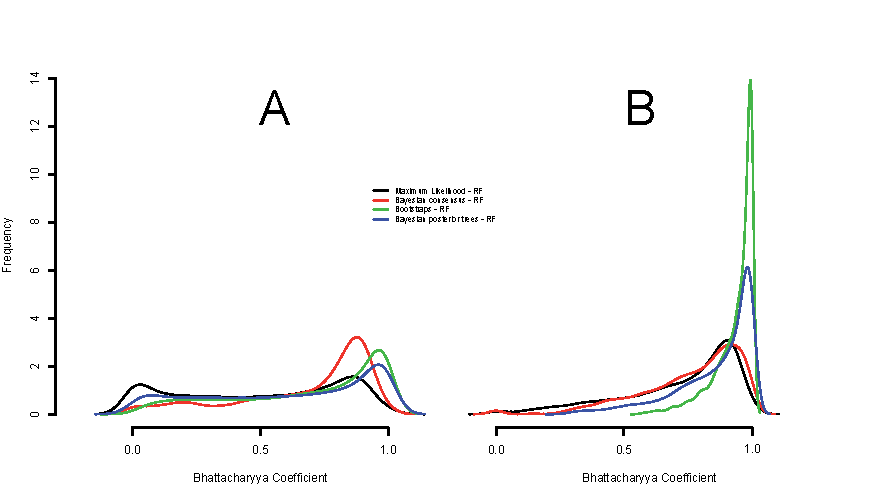
\includegraphics[width=1\textwidth]{SupplementaryMaterial/Supp_Figures/BC-AllMethods-RF+Tr.pdf}
\caption{Distribution of the Pairwise Bhattacharyya Coefficients within each method. A- Distribution of the coefficients when comparing Ronbinson-Foulds distances. B- Distribution of the coefficients when comparing Triplets distances.}
\label{Fig_Bhatt.coeff_distribution} %Differences in overlap within each method
\end{figure}

\begin{figure} 
\centering
    \includegraphics[width=1\textwidth]{SupplementaryMaterial/Supp_Figures/PairwiseComp-ML-RF+Tr.pdf}
\caption{Pairwise Bhattacharyya Coefficients within the Maximum Likelihood trees. The pairwise trees comparisons are represent on both axis. The colour gradient from white to black represents respectively, 0\%, 10\%, 25\%, 50\% and 75\% of missing data for each parameter. The matrix represents the values of pairwise Bhattacharyya Coefficients going from green (1) to red (0). A. Results for the Normalised Robinson-Foulds distance. B. Results with the for Normalised Triplets distance.}
\label{Fig_pairComp-Baytree-RF}
\end{figure} %Pairwise BC for the ML for RF+Tr. (parameters differences)

\begin{figure} 
\centering
    \includegraphics[width=1\textwidth]{SupplementaryMaterial/Supp_Figures/PairwiseComp-Boot-RF+Tr.pdf}
\caption{Pairwise Bhattacharyya Coefficients within the Bootstrap trees. The pairwise trees comparisons are represent on both axis. The colour gradient from white to black represents respectively, 0\%, 10\%, 25\%, 50\% and 75\% of missing data for each parameter. The matrix represents the values of pairwise Bhattacharyya Coefficients going from green (1) to red (0). A. Results for the Normalised Robinson-Foulds distance. B. Results with the for Normalised Triplets distance.}
\label{Fig_pairComp-Baytree-Tr}
\end{figure} %Pairwise BC for the Boot for RF+Tr. (parameters differences)

\begin{figure} 
\centering
    \includegraphics[width=1\textwidth]{SupplementaryMaterial/Supp_Figures/PairwiseComp-Baytre-RF+Tr.pdf}
\caption{Pairwise Bhattacharyya Coefficients within the Bayesian posterior distribution trees. The pairwise trees comparisons are represent on both axis. The colour gradient from white to black represents respectively, 0\%, 10\%, 25\%, 50\% and 75\% of missing data for each parameter. The matrix represents the values of pairwise Bhattacharyya Coefficients going from green (1) to red (0). A. Results for the Normalised Robinson-Foulds distance. B. Results with the for Normalised Triplets distance.}
\label{Fig_pairComp-MLbest-RF}
\end{figure} %Pairwise BC for the Baytre for RF+Tr. (parameters differences)


%Summary of metrics values for all parameters combinations
\begin{table}[ht]
\centering
\begin{tabular}{rrrrrrr}
  \hline
 & Min. & 1st Qu. & Median & Mean & 3rd Qu. & Max. \\ 
  \hline
  Maximum likelihood-RF & 0.06 & 0.26 & 0.40 & 0.41 & 0.50 & 0.95 \\ 
  Maximumlikelihood-Tr & 0.29 & 0.45 & 0.59 & 0.63 & 0.84 & 1.00 \\ 
  Bayesian consensus-RF & 0.69 & 0.71 & 0.72 & 0.76 & 0.79 & 0.96 \\ 
  Bayesian consensus-Tr & -0.28 & -0.11 & 0.17 & 0.19 & 0.37 & 0.98 \\ 
  Bootstraps-RF & 0.06 & 0.18 & 0.27 & 0.26 & 0.34 & 0.46 \\ 
  Bootstraps-Tr & 0.23 & 0.31 & 0.35 & 0.38 & 0.45 & 0.58 \\ 
  Bayesian posterior trees-RF & 0.16 & 0.22 & 0.32 & 0.34 & 0.42 & 0.65 \\ 
  Bayesian posterior trees-Tr & 0.24 & 0.35 & 0.40 & 0.50 & 0.67 & 0.98 \\ 
   \hline
   \hline
\end{tabular}
\end{table}

%Summary of metrics values for the ML parameter
\begin{table}[ht]
\centering
\begin{tabular}{rrrrrrr}
  \hline
 & Min. & 1st Qu. & Median & Mean & 3rd Qu. & Max. \\ 
  \hline
Maximum likelihood-RF & 0.44 & 0.51 & 0.63 & 0.66 & 0.78 & 0.95 \\ 
  Maximumlikelihood-Tr & 0.45 & 0.56 & 0.76 & 0.74 & 0.93 & 0.99 \\ 
  Bayesian consensus-RF & 0.71 & 0.73 & 0.80 & 0.82 & 0.88 & 0.95 \\ 
  Bayesian consensus-Tr & 0.37 & 0.46 & 0.67 & 0.67 & 0.87 & 0.96 \\ 
  Bootstraps-RF & 0.34 & 0.37 & 0.42 & 0.41 & 0.44 & 0.46 \\ 
  Bootstraps-Tr & 0.32 & 0.40 & 0.51 & 0.46 & 0.51 & 0.57 \\ 
  Bayesian posterior trees-RF & 0.33 & 0.41 & 0.52 & 0.50 & 0.60 & 0.65 \\ 
  Bayesian posterior trees-Tr & 0.41 & 0.56 & 0.76 & 0.71 & 0.84 & 0.98 \\ 
   \hline
\end{tabular}
\end{table}

%Summary of metrics values for the ML parameter
\begin{table}[ht]
\centering
\begin{tabular}{rrrrrrr}
  \hline
 & Min. & 1st Qu. & Median & Mean & 3rd Qu. & Max. \\ 
  \hline
Maximum likelihood-RF & 0.23 & 0.46 & 0.64 & 0.61 & 0.79 & 0.93 \\ 
  Maximumlikelihood-Tr & 0.65 & 0.84 & 0.95 & 0.89 & 0.99 & 1.00 \\ 
  Bayesian consensus-RF & 0.72 & 0.77 & 0.86 & 0.85 & 0.94 & 0.96 \\ 
  Bayesian consensus-Tr & -0.16 & 0.19 & 0.63 & 0.52 & 0.96 & 0.98 \\ 
  Bootstraps-RF & 0.14 & 0.30 & 0.40 & 0.35 & 0.45 & 0.46 \\ 
  Bootstraps-Tr & 0.37 & 0.49 & 0.54 & 0.51 & 0.56 & 0.57 \\ 
  Bayesian posterior trees-RF & 0.24 & 0.45 & 0.57 & 0.51 & 0.63 & 0.65 \\ 
  Bayesian posterior trees-Tr & 0.44 & 0.81 & 0.86 & 0.82 & 0.98 & 0.98 \\ 
   \hline
\end{tabular}
\end{table}

%Summary of metrics values for the MC parameter
\begin{table}[ht]
\centering
\begin{tabular}{rrrrrrr}
  \hline
 & Min. & 1st Qu. & Median & Mean & 3rd Qu. & Max. \\ 
  \hline
Maximum likelihood-RF & 0.40 & 0.50 & 0.64 & 0.65 & 0.79 & 0.94 \\ 
  Maximumlikelihood-Tr & 0.70 & 0.84 & 0.93 & 0.89 & 0.99 & 1.00 \\ 
  Bayesian consensus-RF & 0.76 & 0.79 & 0.86 & 0.86 & 0.92 & 0.96 \\ 
  Bayesian consensus-Tr & 0.05 & 0.16 & 0.53 & 0.50 & 0.87 & 0.92 \\ 
  Bootstraps-RF & 0.25 & 0.34 & 0.42 & 0.38 & 0.45 & 0.46 \\ 
  Bootstraps-Tr & 0.38 & 0.47 & 0.55 & 0.51 & 0.57 & 0.58 \\ 
  Bayesian posterior trees-RF & 0.32 & 0.44 & 0.58 & 0.52 & 0.62 & 0.65 \\ 
  Bayesian posterior trees-Tr & 0.39 & 0.78 & 0.82 & 0.79 & 0.98 & 0.98 \\ 
   \hline
\end{tabular}
\end{table}


%Summary of the BC between pairs of methods for the ML parameter
\begin{table}[ht]
\centering
\begin{tabular}{rrrrrrr}
  \hline
 & Min. & 1st Qu. & Median & Mean & 3rd Qu. & Max. \\ 
  \hline
Maximum.likelihood.vs..Bayesian.consensus...RF & 0.30 & 0.31 & 0.69 & 0.61 & 0.77 & 1.00 \\ 
  Maximum.likelihood.vs..Bayesian.consensus...Tr & 0.79 & 0.81 & 0.84 & 0.86 & 0.85 & 1.00 \\ 
  Maximum.likelihood.vs..Bootstraps...RF & 0.03 & 0.22 & 0.29 & 0.36 & 0.54 & 0.69 \\ 
  Maximum.likelihood.vs..Bootstraps...Tr & 0.08 & 0.42 & 0.53 & 0.51 & 0.74 & 0.78 \\ 
  Maximum.likelihood.vs..Bayesian.posterior.trees...RF & 0.02 & 0.49 & 0.61 & 0.51 & 0.67 & 0.74 \\ 
  Maximum.likelihood.vs..Bayesian.posterior.trees...Tr & 0.21 & 0.61 & 0.70 & 0.63 & 0.81 & 0.81 \\ 
  Bayesian.consensus.vs..Bootstraps...RF & 0.01 & 0.02 & 0.02 & 0.02 & 0.03 & 0.04 \\ 
  Bayesian.consensus.vs..Bootstraps...Tr & 0.08 & 0.69 & 0.78 & 0.64 & 0.79 & 0.84 \\ 
  Bayesian.consensus.vs..Bayesian.posterior.trees...RF & 0.01 & 0.02 & 0.02 & 0.04 & 0.08 & 0.09 \\ 
  Bayesian.consensus.vs..Bayesian.posterior.trees...Tr & 0.21 & 0.74 & 0.75 & 0.68 & 0.84 & 0.87 \\ 
  Boostraps.vs..Bayesian.posterior.trees...RF & 0.69 & 0.75 & 0.85 & 0.85 & 0.95 & 1.00 \\ 
  Boostraps.vs..Bayesian.posterior.trees...Tr & 0.91 & 0.92 & 0.96 & 0.95 & 0.97 & 0.98 \\ 
   \hline
\end{tabular}
\end{table}

%Summary of the BC between pairs of methods for the MF parameter
\begin{table}[ht]
\centering
\begin{tabular}{rrrrrrr}
  \hline
 & Min. & 1st Qu. & Median & Mean & 3rd Qu. & Max. \\ 
  \hline
Maximum.likelihood.vs..Bayesian.consensus...RF & 0.00 & 0.25 & 0.48 & 0.50 & 0.76 & 1.00 \\ 
  Maximum.likelihood.vs..Bayesian.consensus...Tr & 0.38 & 0.69 & 0.75 & 0.72 & 0.80 & 1.00 \\ 
  Maximum.likelihood.vs..Bootstraps...RF & 0.03 & 0.18 & 0.32 & 0.36 & 0.47 & 0.77 \\ 
  Maximum.likelihood.vs..Bootstraps...Tr & 0.08 & 0.34 & 0.40 & 0.38 & 0.53 & 0.55 \\ 
  Maximum.likelihood.vs..Bayesian.posterior.trees...RF & 0.02 & 0.47 & 0.71 & 0.60 & 0.86 & 0.94 \\ 
  Maximum.likelihood.vs..Bayesian.posterior.trees...Tr & 0.21 & 0.54 & 0.62 & 0.56 & 0.64 & 0.80 \\ 
  Bayesian.consensus.vs..Bootstraps...RF & 0.00 & 0.00 & 0.01 & 0.01 & 0.01 & 0.03 \\ 
  Bayesian.consensus.vs..Bootstraps...Tr & 0.08 & 0.38 & 0.54 & 0.49 & 0.70 & 0.75 \\ 
  Bayesian.consensus.vs..Bayesian.posterior.trees...RF & 0.00 & 0.02 & 0.02 & 0.02 & 0.04 & 0.04 \\ 
  Bayesian.consensus.vs..Bayesian.posterior.trees...Tr & 0.21 & 0.29 & 0.66 & 0.54 & 0.72 & 0.82 \\ 
  Boostraps.vs..Bayesian.posterior.trees...RF & 0.69 & 0.69 & 0.72 & 0.71 & 0.72 & 0.72 \\ 
  Boostraps.vs..Bayesian.posterior.trees...Tr & 0.91 & 0.91 & 0.91 & 0.93 & 0.92 & 0.98 \\ 
   \hline
\end{tabular}
\end{table}

%Summary of the BC between pairs of methods for the MC parameter
\begin{table}[ht]
\centering
\begin{tabular}{rrrrrrr}
  \hline
 & Min. & 1st Qu. & Median & Mean & 3rd Qu. & Max. \\ 
  \hline
Maximum.likelihood.vs..Bayesian.consensus...RF & 0.03 & 0.32 & 0.66 & 0.55 & 0.75 & 1.00 \\ 
  Maximum.likelihood.vs..Bayesian.consensus...Tr & 0.51 & 0.69 & 0.80 & 0.76 & 0.80 & 1.00 \\ 
  Maximum.likelihood.vs..Bootstraps...RF & 0.03 & 0.17 & 0.21 & 0.31 & 0.46 & 0.68 \\ 
  Maximum.likelihood.vs..Bootstraps...Tr & 0.08 & 0.31 & 0.39 & 0.39 & 0.56 & 0.61 \\ 
  Maximum.likelihood.vs..Bayesian.posterior.trees...RF & 0.02 & 0.44 & 0.47 & 0.52 & 0.78 & 0.90 \\ 
  Maximum.likelihood.vs..Bayesian.posterior.trees...Tr & 0.21 & 0.52 & 0.59 & 0.55 & 0.66 & 0.77 \\ 
  Bayesian.consensus.vs..Bootstraps...RF & 0.00 & 0.01 & 0.01 & 0.02 & 0.02 & 0.03 \\ 
  Bayesian.consensus.vs..Bootstraps...Tr & 0.08 & 0.47 & 0.62 & 0.51 & 0.66 & 0.73 \\ 
  Bayesian.consensus.vs..Bayesian.posterior.trees...RF & 0.00 & 0.02 & 0.04 & 0.04 & 0.05 & 0.06 \\ 
  Bayesian.consensus.vs..Bayesian.posterior.trees...Tr & 0.21 & 0.45 & 0.64 & 0.57 & 0.74 & 0.79 \\ 
  Boostraps.vs..Bayesian.posterior.trees...RF & 0.69 & 0.73 & 0.73 & 0.76 & 0.81 & 0.86 \\ 
  Boostraps.vs..Bayesian.posterior.trees...Tr & 0.91 & 0.92 & 0.93 & 0.94 & 0.96 & 0.99 \\ 
   \hline
\end{tabular}
\end{table}
  \label{Supp_results}

%END
\end{document}
    \label{SupplementaryMaterial}


%END
\end{document}